% modificar la caratula

% falta analisis de resultados (que despues se replica en las conclusiones) ¿Que mas se puede poner?

% concluciones: presentamos una herramienta, analizamos los ejemplos para ver la ganacia obteniendo una mejora de 10 veces.
\documentclass[a4paper,	11pt]{report}
%-----------Paquetes-------------------------
\usepackage[utf8]{inputenc}
\usepackage{amsmath}
\usepackage{amssymb}
\usepackage{minted}
\usepackage{todonotes}

\usepackage{xpatch,letltxmacro}
\LetLtxMacro{\cminted}{\minted}
\let\endcminted\endminted
\xpretocmd{\cminted}{\RecustomVerbatimEnvironment{Verbatim}{BVerbatim}{}}{}{}


\usemintedstyle{trac} 
\usepackage[hidelinks]{hyperref}
%\usepackage[lined,boxed,spanish,onelanguage]{algorithm2e} 
\usepackage{algorithm}
\usepackage{algpseudocode}
\usepackage{graphicx}
\usepackage[strict]{changepage}

\usepackage{booktabs}
\usepackage[outermargin=-4cm,]{fullwidth}
\usepackage{tikz}
\usetikzlibrary{trees}

\tikzstyle{every node}=[draw=black,thick,anchor=west]
\tikzstyle{selected}=[draw=red,fill=red!30]
\tikzstyle{optional}=[dashed,fill=gray!50]

\usepackage{mdframed}

\usepackage[spanish]{babel}
\renewcommand\listingscaption{Listado}

\newcommand\TBox[2][]{%
  \tikz\node[draw,ultra thick,align=left,#1] {#2};\hskip2pt}

\begin{document}

\renewcommand\floatpagefraction{.9}
\renewcommand\topfraction{.9}
\renewcommand\bottomfraction{.9}
\renewcommand\textfraction{.1}
\setcounter{totalnumber}{50}
\setcounter{topnumber}{50}
\setcounter{bottomnumber}{50}
\newcommand{\quotes}[1]{``#1''}

\title{Conversión de modelos PowerDEVS al lenguaje Modelica}
\author{Tesinista: Luciano Andrade A-2121/1\\ Director: Federico Bergero, Co-Director: Ernesto Kofman} 


\begin{titlepage}
\begin{center}

\huge Conversión de modelos PowerDEVS al lenguaje Modelica

\vfill

Tesina de grado para la obtención del grado de Licenciado en Ciencias de la Computación

\begin{minipage}[t]{0.4\textwidth}
\begin{flushleft} \large
\emph{Tesinista :}\\
Luciano Andrade
\end{flushleft}
\end{minipage}\\ 
\vfill
\begin{minipage}[t]{0.4\textwidth}
\begin{flushleft} \large
\emph{Director :}\\
Federico Bergero
\end{flushleft}
\end{minipage}%
\begin{minipage}[t]{0.4\textwidth}
\begin{flushright} \large
\emph{Co-Director:} \\
Ernesto Kofman 
\end{flushright}
\end{minipage}

\vfill


\includegraphics[width=0.25\textwidth]{logo-unr}

\vfill

{\large \today}
\end{center}
\end{titlepage}


\tableofcontents

\begin{abstract}

El modelado y simulación se han convertido en una actividad centrales de todas las disciplina ingenieriles y científicas, son utilizados en el análisis de sistemas  ayudándonos a ganar un mejor entendimiento de su funcionamiento. 
Son importantes para el diseño de nuevos sistemas donde podemos predecir el comportamiento del sistema antes de que sea construido.
El modelado y simulación son las únicas técnicas disponibles que nos permiten analizar sistemas arbitrarios no lineales bajo una variedad de condiciones experimentales.

PowerDEVS es un entorno integrado para el modelado y simulación basada en el formalismo DEVS, permite definir modelos atómico en C++ que puede ser conectados gráficamente en bloques jerárquicos para crear sistemas más complejos. El entorno automáticamente transforma el modelo a código C++ que ejecuta la simulación.

\todo[inline]{Desperdician no es la palabra correcta, si no que en el caso de la simualación continnua muchas cosas no hacen falta que en DEVS sí}
QSS-Solver es una implementación de los métodos de integración por cuantificación de estados (Quantized State System) los cuales permiten, a diferencia de las implementaciones sobre eventos discretos no desperdician carga computacional en la simulación de eventos discretos.

\todo[inline]{Falta decir qué vas a hacer en este trabajo. Introducís "esta herramienta" y no se entiende qué herramienta}
Esta herramienta convierte los modelos, descriptos en PowerDEVS, en código Modelica, más especificamente código $\mu$-Modelica (un subconjunto de Modelica), permitiendo ejecutar este modelo (convertido) con alguno de los compiladores Modelica, OpenModelica o Dymola, o \quotes{QSS Solver}, este último nos permite ganar al menos un orden de magnitud en los tiempos incurridos en la simulación.

\end{abstract}


\chapter{Introducción}
\section{Motivación}
El modelado y simulación se han convertido en una actividad centrales de todas las disciplina ingenieriles y científicas, son utilizados en el análisis de sistemas  ayudándonos a ganar un mejor entendimiento de su funcionamiento. 

Son importantes para el diseño de nuevos sistemas donde podemos predecir el comportamiento del sistema antes de que sea construido.
El modelado y simulación son las únicas técnicas disponibles que nos permiten analizar sistemas arbitrarios no lineales bajo una variedad de condiciones experimentales.

Veamos algunas razones por las cuales utilización de simulaciones es deseable o incluso requerido:

\begin{itemize}
	\item El sistema físico no se encuentra disponible, se debido a que el sistema no fue aun construido o si el sistema debería ser construido. 
	
	\item El experimento puede ser peligroso. Usualmente, simulaciones son realizadas para determinar si el experimento real \quotes{explotara}, poniendo al experimentador en peligro.

	\item El costo del experimento es demasiado alto o las herramientas necesarias no se encuentran disponibles o son muy costosas. Tambien es posible que el sistema se encuentra siendo utilizado y tomar el tiempo para experimentar sería inaceptable.

	\item Los tiempos del sistema no son compatibles con el del experimentador. Usualmente simulaciones son utilizadas debido a que el experimento real se realiza tan rapido que no es posible observarlo (por ejemplo una explosión) o porque el experimento toma tanto tiempo que el experimmentador estaria muerto cuando el experimento se encuentre completado.

	\item Variables de control, de estado y/o del sistema pueden encontrarse inaccesibles. Usualmente simulaciones son utilizadas debido a que nos permite acceder todas las variables de entrada y todos los estados, mientras que el sistema real, algunas entradas ( ruidos, por ejemplo) no son manipulables y algunas variables internas del sistema no son accesibles a la medición. Simulaciones tambien nos permite manipular el modelo en formas que no podriamos manipular el sistema real, por ejemplo, podemos decidir cambiar la masa de un objeto de 50 kg a 400 kg y repetir la simulación. En un sistema físico, la modificación anterior es imposible o requiere una costoza y larga alteración del sistema.

	\item Eliminación de perturbaciones. Usualmente, se llevan adelante simulaciones que nos permite eliminar perturbaciones que son inevitables en el sistema real. Lo que nos permite aislar efectos particulares, y puede conducir a mejores apreciaciones sobre el comportamiento general del sistema.

	\item Eliminación de efectos de segundo orden. Usualmente, se utilizan simulaciones porque nos permite eliminar efectos de segundo orden (como no linealidades de componentes del sistema). Nuevamente esto ayuda a obtener un mejor entendimiento del comportamiento general del sistema.
\end{itemize}

Es por esto que cuando corremos un modelo es deseable que pueda ser simulado de la forma más rapida y eficiente posible.

Para realizar la simulación debemos generar el modelo, es decir, la descripción de nuestro sistema de forma que sea posible compilarse en código de maquina para poder ser ejecutado (pasando por un lenguaje de propósito general, usualmente C o C++). 

El modelo generamente inicia como una función matemática de la forma 
\begin{equation*}
	\dot{x} = f(x, u, t)
\end{equation*}
donde $x$ representan las variables del sistema, $u$ el estado inicial y $t$ el tiempo, este modelo, puede ser convertido en un modelo Modelica de forma textual o gráfica, dependiendo de las herramientas con las que contemos y como nos resulte más simple de describir.

PowerDEVS\cite{BK11} es una herramienta de simulación de sistemas híbridos, basado en el formalismo DEVS\cite{Zeigler:2000:TMS:580780}, con una interfaz gráfica orientada a bloques, donde los bloques pueden ser conectados entre si, modificado sus parámetros, además permite conectarse con el entorno Scilab para poder utilizar expresiones y herramientas de cálculo provistas por este entorno.

Nos interesa poder utilizar el entorno PowerDEVS, debido a que no solo la interfaz gráfica es más amena para usuarios que no estan necesariamente habituados a la programación, sino que tambien deseamos utilizar los modelos ya definidos en esta herramienta.

En este aspecto, contamos con la herramienta \quotes{QSS-Solver}, la cual nos permitiria ejectura simulaciones un orden de mágnitud más rápido, que otras implementaciones.

Por lo cual enn este trabajo nos proponemos mostrar una aplicación capaz de convertir modelos descriptos en la herramienta PowerDEVS\cite{BK11} a modelos en el lenguaje Modelica\cite{Fritzson02modelica--}, más específicamente en $\mu$Modelica\cite{Ber12}, capaz de ser ejecutados en el QSS-Solver, obteniendo lo mejor de los dos mundos.


\begin{figure}[H]
\centering
 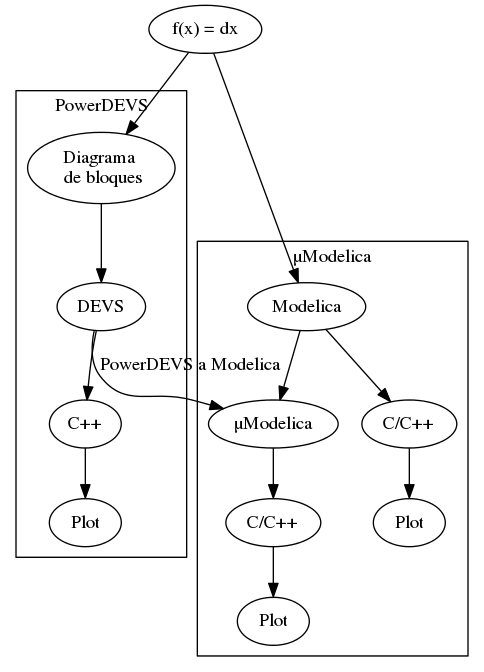
\includegraphics[width=0.75\linewidth]{esquema}
 \caption{Esquema de conversiones}
 \label{fig:esquema}
\end{figure}

En la figura \ref{fig:esquema}, se muestran los dos principales estrategias (PowerDEVS y Modelica) para realizar una simulación. En el caso de PowerDEVS, el primer paso es convertir el sistema en diagramas de bloques, luego en DEVS, en PowerDEVSe el cual puede automáticamente convertirlo en C++ y luego obtener los resultados ejecutando este modelo. 

Desde la perspectiva de Modelica (o $\mu$-Modelica), debemos pasar el sistema a Modelica (o $\mu$-Modelica) y luego el compilador se encargara de generar código (usualmente C o C++) capaz de correr la simulación y obtener resultados.

El actual trabajo está representado por la flecha que sale de PowerDEVS hacia $\mu$modelica, permitiendo especificar la simulación en diagramas de bloques y ejecutar la simulación en el QSS-Solver, en el lenguaje $\mu$modelica.

\section{Organización del trabajo}
El presente trabajo se organiza en 6 capítulos:
\begin{itemize}
\item \emph{Introducción} en la cual ya vimos una visión general del objetivo así como las herramientas que utilizaremos y algunas herramientas relacionadas
\item \emph{Conceptos previos} en este capítulo veremos los fundamentos matemáticos y profundizaremos sobre las dos herramientas principales que conciernen este trabajo.
\item \emph{Conversión de modelos DEVS} en este capítulo veremos en detalles la conversión de un modelo desde su formulación matemática, en su modelo en PowerDEVS y veremos las conversiones necesarias para llevar adelante la conversión a $\mu$-Modelica.
\item \emph{Detalles de la implementación} en este capítulo se muestra los componentes de software que forman la aplicación, y descripción en pseudo-código de los principales componentes.
\item \emph{Ejemplos y Resultados} en este capítulo vemos varios ejemplos y realizamos una comparación de los resultados obtenidos a partir de compara los tiempos de simulaciones de los modelos originales, en PowerDEVS, y los modelos convertidos en $\mu$-Modelica.
\item \emph{Conclusiones}, por último revisamos nuestras conclusiones y proponemos trabajos a futuro.
\end{itemize}

\section{Trabajo relacionado}
En \cite{Ber12} se describe una extensión del Compilador OpenModelica el cual traslada modelos regulares Modelica a un subconjunto más simple $\mu$-Modelica, el cual puede ser interpretado directamente por el QSS-Solver.


ModelicaDEVS \cite{Beltrame06quantisedstate} es una librería Modelica que permite describir simulaciones DEVS, ofrece una re-implementación de PowerDEVS dentro del marco de Modelica.

DESlib \cite{Sanz09paralleldevs} es una librería para la descripción de modelos Parallel DEVS y Modelado orientado a proceso en Modelica.
La librería contiene cuatro paquetes que pueden ser utilizados para modelar sistemas de eventos discretos:
\begin{itemize}
\item RandomLib puede generar números y variables aleatorias, siguiendo distribuciones de probabilidades discretas y continuas.
\item DEVSLib puede ser utilizado para modelar sistemas de eventos discretos (DEVS) siguiendo el formalismo de parallel DEVS.
\item SIMANLib y ARENALib puede ser utilizado para modelar sistemas de eventos discretos (DEVS) siguiendo el enfoque orientado al proceso.
\end{itemize}

Estas dos librerías llevan los formalismos DEVS hacia Modelica, pero no utilizan la herramienta powerdevs, ni se ejecutan en QSS-Solver.
Podríamos desarrollar los modelos utilizando estas librerías y ejecutar la simulación del modelo convertido en $\mu$-Modelica con el QSS-Solver, pero esto no permite re-utilizar los modelos desarrollados en PowerDEVS.


M/CD++ \cite{conf/mascots/DAbreuW05} es una herramienta para convertir simulaciones en un subconjunto de Modelica, a simulaciones DEVS, este trabajo funciona en sentido opuesto a nuestro trabajo, es decir convirtiendo modelos Modelica en modelos DEVS, por lo que no utiliza PowerDEVS y no ejecuta la simulación en el QSS-Solver.



\chapter{Conceptos Previos}
	En este capítulo, basado en \cite{Fer12}, \cite{Ber12Th}, \cite{BK11}, \cite{BK13}, introducimos algunos conceptos básicos de modelado y 
	simulación de sistemas, formalismos necesarios para poder comprender este trabajo. 

\section{Modelado y Simulación}
	El Modelado y Simulación\cite{Zeigler} de un Sistema es el proceso por el cual se desarrolla un modelo, el cual es luego ejecutado, de forma de obtener datos 
	sobre el comportamiento del sistema.  El modelo debe conservar las principales características del sistema, pero al mismo tiempo ser significativamente 
	más simple, de forma que al momento de simularlo sea más eficaz utilizar la simulación que el sistema en sí.

	\subsection{Sistemas Continuos y Discretos}
	Se considera un sistema continuo si las variables de éste son conocidas en cada instante de tiempo, mientras que se considera discreto si las 
	variables son conocidas en instantes de tiempo determinados.

	En general, los sistemas en estudio serán continuos, pero deberemos utilizar sistemas discretos para simularlo, puésto que la simulación en 
	computadora así lo requiere, dado que la misma computadora es un sistema discreto.

	\subsection{Métodos de Integración numérica} \label{sec:num_integ}
	Un sistema continuo puede ser descripto por un modelo en espacios de estados de la forma:

	\begin{equation} \label{eq:eq1}
	\dot{x}(t) = f (x(t), u(t))
	\end{equation}

	donde $x \in \mathbb{R}^n$  es el vector de estados, $u \in \mathbb{R}^m$ es una función de entradas conocidas,
	$t$ representa el tiempo y con sus condiciones iniciales:

	\begin{equation} \label{eq:eq2}
	x(t = t_0 ) = x_0
	\end{equation}

	Sea $x_i (t)$ la trayectoria del estado $i$-esimo expresada como función de tiempo simulado. 
	Mientras que la ecuación  \eqref{eq:eq1} no contenga discontinuidades $x_i (t)$ será una función continua con derivada continua. 
	Esta puede ser aproximada con la precisión deseada mediante series de Taylor en cualquier punto de su trayectoria.

	Denominando $t^{\ast}$ al instante de tiempo en torno al cual se aproxima la trayectoria mediante una serie de Taylor, y siendo $t^{\ast} + h$
	 el instante de tiempo en el cual se quiere evaluar la aproximación, entonces, la trayectoria en dicho punto puede expresarse como sigue:

	\begin{equation} \label{eq3}
		x_i(t^* + h) = x_i(t^*) + \frac{dx_i (t^*)}{dt} \cdot h + \frac{d^{2}x_i (t^*)}{dt^2} \cdot \frac{h^2}{2!} + \cdots
	\end{equation}

	Reemplazando con la ecuación de estado \ref{eq:eq1}, la serie \eqref{eq3} queda:

	\begin{equation} \label{eq4}
		x_i(t^* + h) = x_i(t^*) + f_i(t^*) \cdot h + \frac{d^{2}x_i (t^*)}{dt^2} \cdot \frac{h^2}{2!} + \cdots
	\end{equation}

	Los distintos algoritmos de integración difieren en la manera de aproximar las derivadas superiores de $f$ y en el número de
	 términos de la serie de Taylor que consideran para la aproximación, entre los principales métodos podemos mencionar Runge-Kutta, DASSL, DOPRI, etc.

	A modo de ejemplos introducimos un ejemplo: el sistema de ecuaciones de Lotka-Volterra, también conocidas como ecuaciones predador-presa o presa-predador,
	son un par de ecuaciones diferenciales de primer orden no lineales que se usan para describir la dinámicas de sistemas biológicos en el que dos 
	especies interactúan, una como presa y otra como depredador.

	\begin{align*}
		\frac{dx}{dt} &= x(\alpha - \beta y) \\
		\frac{dy}{dt} &= - y(\gamma - \delta  x)
	\end{align*}

	donde:
	\begin{itemize}
		\item $y$ es el número de algún predador (por ejemplo, un lobo)
		\item $x$ es el número de sus presas (por ejemplo, conejos)
		\item $\frac{dy}{dt}$ y $\frac{dx}{dt}$ representa el crecimiento de las dos poblaciones en el tiempo
		\item t representa el tiempo y
		\item $\alpha$, $\beta$, $\gamma$ y $\delta$ son parámetros que representan las interacciones de las dos especies.
	\end{itemize}

\section{Modelica}

	Modelica\cite{Fri98}\cite{Fritzson02modelica} es un lenguaje orientado a objetos desarrollado para describir de manera sencilla modelos de sistemas 
	dinámicos eventualmente muy complejos.
	Además de las características básicas de todo lenguaje orientado a objetos, contiene herramientas específicas que permiten describir las relaciones
	constitutivas de los distintos componentes de cada modelo y las relaciones estructurales que definen la interacción entre dichos componentes.
	De esta manera, el lenguaje permite asociar cada componente de un sistema a una instancia de una clase.
	Adicionalmente, los componentes típicos de los sistemas de distintos dominios de la física y de la técnica pueden agruparse en librerías de clases para ser
	reutilizados. De hecho, existe una librería estándar de clases de Modelica, que contiene los principales componentes básicos de sistemas eléctricos,
	mecánicos (traslacionales, rotacionales y multicuerpos), térmicos, state graphs, y diagramas de bloques. 
	Otras librerías (disponibles en la web) contienen componentes de sistemas hidráulicos, bond graphs, redes de petri, etc.
	Por otro lado, las herramientas que provee Modelica para expresar relaciones estructurales de un modelo permiten construir la estructura del mismo de una
	manera totalmente gráfica, lo que a su vez permite describir un sistema mediante un diagrama muy similar al del Sistema Físico Idealizado.
	Como con todo lenguaje, para poder simular un modelo descripto en Modelica es necesario utilizar un compilador. Actualmente existen tres compiladores
	más o menos completos de Modelica: Dymola, MathModelica y OpenModelica. Los dos primeros son herramientas comerciales que cuentan con interfaces
	gráficas para construir los modelos. OpenModelica es una herramienta libre, de código abierto.

\begin{listing}[H]    
	\caption{LotkaVolterra.mo}
	\inputminted[linenos]{modelica}{src/LotkaVolterra.mo}
	\label{lst:LotkaVolterra.mo}
\end{listing}
	
	Continuando con el ejemplo del sistema de ecuaciones de Lotka-Volterra, en el listado \ref{lst:LotkaVolterra.mo} se muestra el equivalente modelo en Modelica, 
	en el se pueden observar algunas particularidades del lenguaje.
	
	En la primera linea se puede ver que el modelo, en este caso una \quotes{clase}, y su nombre LotkaVolterra.
	Modelica, utiliza 7 clases restringidas:
	\textbf{block}, \textbf{connector}, \textbf{function}, \textbf{model}, \textbf{package}, \textbf{record} y \textbf{type}.
	Cada una de estas clases restringidas permite declarar clases más específicas cualquiera de ellas puede reemplazarse
	por \textbf{class}, pero siempre es mejor especificar de que tipo de clase se trata para mejorar la legibilidad y facilitar la depuración de código.

	Las siguientes dos lineas declaran las variables \texttt{x} e \texttt{y} del tipo \texttt{Real}, ambas con valor de inicio \texttt{0.5}, las lineas 4 a 7, 
	declaran los parámetros \texttt{a}, \texttt{b}, \texttt{c} y \texttt{d} a diferencia de \texttt{x} e \texttt{y}, estos parámetros no pueden cambiar durante la 
	simulación, pero pueden cambiar de simulación en simulación.

	Esta primera parte (lineas 2 a 7) del modelo constituye la sección de declaraciones, se encuentra la sección de ecuaciones (luego de la palabra clave 
	\texttt{equation}), esta sección describe el sistema de ecuaciones de nuestro modelo. Donde la expresión \texttt{der(x)} representa la derivada \texttt{x} 
	respecto del tiempo y análogamente con \texttt{y}.
	Es importante notar que el símbolo \texttt{=} no es el símbolo de asignación, sino de igualdad matemática (es decir acausal), a diferencia de la mayoría 
	de  los lenguajes de programación modernos.  Para realizar asignaciones se utiliza una sección \texttt{algorithm}, que contiene asignaciones ordenadas. 
	Con el fin de distinguir de las ecuaciones de la sección \texttt{equation}, se utiliza el operador de asignación \texttt{:=}, 
	varias asignaciones puede ser ejecutadas en la sección de \texttt{algorithm}. Ademas la sección \texttt{algorithm} puede tener expresiones y construcciones 
	if-then-else y bucles.

	Por supuesto Modelica es un lenguaje mucho más extenso de lo que hemos descripto, pero los conceptos que utilizamos a lo largo de este trabajo son los
	expresados en la presente sección.


\section{Métodos de integración QSS}
	Los métodos Quantized State System \cite{Fer12}, \cite{Ber12}, \cite{Beltrame06quantisedstate}, \cite{Cel06}, pueden aproximar Ecuaciones 
	Diferenciales Ordinarias (ODE por sus siglas en inglés) mediante modelos de eventos discretos cuantificando los estados del sistema, 
	a diferencia de los métodos mencionados en la sección \ref{sec:num_integ}, los cuales realizan la integración sobre el tiempo. 

	Formalmente, el método de QSS de primer orden (llamado QSS1) aproxima la ecuación por:
	
	\begin{equation}
	\dot{x}(t) = f (q(t), v(t))
	\end{equation}
	
	donde $q$ es el vector de estados cuantificados y sus componentes están relacionadas una a una con las del vector de estados $x$ siguiendo una 
	función de cuantificación con histéresis:
	
	\begin{equation}
	q_j(t) = \left\{ 
	  \begin{array}{l l}
	    x_j(t)  \quad \text{si} \mid x_j (t ) - q_j (t^{-} ) \mid \geq \Delta Q_j \\
	    q_j (t^{-} ) \quad \text{en caso contrario}
	  \end{array} \right.
	\end{equation}
	
	donde $q_j (t^{-})$ es el límite por izquierda de $q_j$ en $t$.
	
	\begin{figure}[!htbp]
	  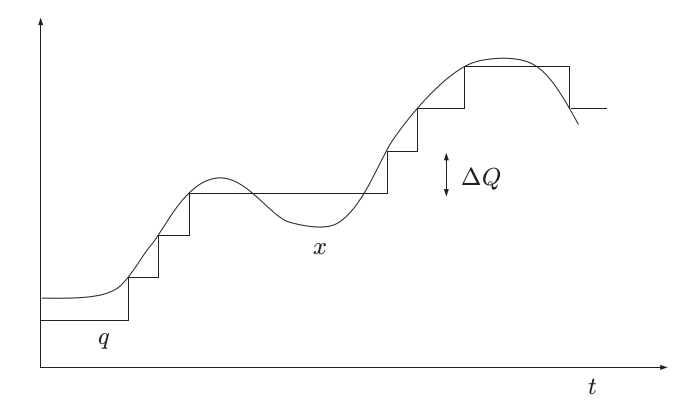
\includegraphics[scale=0.5]{histeresis1}
	  \caption{Comportamiento de un modelo DEVS atómico}
	   \label{fig:fig2-2}
	\end{figure}
	
	En la Figura \ref{fig:fig2-2} vemos la relación entrada-salida de una función de cuantificación de orden cero.
	
	Las variables $q_j$ son llamadas variables cuantificadas y pueden ser vistas como una aproximación constante a trozos de la variable de estado 
	correspondiente $x_j$. De la misma forma las componentes de $v(t)$ son aproximaciones constantes a trozos de las componentes correspondientes de $u(t)$. 
	Los pasos de integración en los métodos de QSS sólo se producen cuando una variable cuantificada $q_j (t)$ cambia, esto es, cuando la variable de 
	estado correspondiente $x_j (t)$ difiere de $q_j(t^{-})$ en un quantum. Ese cambio implica también que algunas derivadas de estado (aquellas que 
	dependen de $x_j$ ) también son modificadas. 

	Luego, cada paso involucra un cambio en sólo una variable cuantificada y en algunas derivadas de estado. 
	Por lo tanto cuando un gran sistema ralo (o sparse) posee sólo actividad en unos pocos estados mientras que el resto del sistema se mantiene 
	intacto, los métodos de QSS explotan intrínsecamente este hecho realizando cálculos sólo donde y cuando ocurren los cambios.
	Otra ventaja importante de los métodos de QSS es que tratan las discontinuidades de una manera muy eficiente. Dependiendo del orden del método, 
	las variables de estado siguen trayectorias lineal a trozos, parabólica a trozos o constante a trozos, la ocurrencia de una discontinuidad implica 
	sólo algunos cálculos locales para re-computar las derivadas de estados que están directamente afectadas por ese evento.
	Estas ventajas resultan en una aceleración notable en el tiempo de simulación contra los algoritmos de integración numérica clásicos. 
	En modelos con discontinuidades frecuentes como sistemas de electrónica de potencia, los métodos de alto orden que veremos a continuación, 
	pueden simular hasta 20 veces más rápido que los métodos convencionales.


\section{$\mu$-Modelica}
	El lenguaje $\mu$-Modelica\cite{Ber12} tiene las siguientes restricciones con respecto a Modelica:

	\begin{itemize}
	 \item El modelo es plano, es decir no permite clases.
	 \item Todas las variables pertenecen al tipo predefinido Real y solo hay tres categorías de variables: estado continuo, estado discreto y variables 
	algebraicas.
	 \item Los parámetros también son de tipo Real. 
	 \item Arreglos están permitidos. Indices en los arreglos dentro de cláusulas \texttt{for} están restringidos a la forma $\alpha \cdot i + \beta$, 
	donde $\alpha$ y $\beta$ son expresiones enteras y \texttt{i} es el índice de la iteración.
	 \item La sección de ecuaciones está compuesta de :
	 \begin{itemize}
		\item Definición de variables de estados : $der(x) =  f (x(t), d, a(t), t);$ ODE en forma explícita
		\item Definición algebraica : $(a_1 , \dots , a_n ) = g(x(t), d, a(t), t);$
	 \end{itemize}
	 con la restricción de que cada variable algebraica solo puede depender del estado y de variables algebraicas previamente definidas.
	 
	 \item Discontinuidades son expresadas solo con las clausulas $when$ y $elsewhen$ dentro de la sección $algorithm$. Las condiciones dentro de las dos 
	clausulas solo pueden ser relaciones ($<$, $\leqslant$, $>$ $\geqslant$) y, dentro de la clausula, solo asignaciones de variables discretas y $reinit$ 
	de estados continuos son permitidos.
	\end{itemize}

\section{Stand–Alone QSS solver}
	Como mencionamos antes los métodos QSS de integración remplazan la discretización del tiempo de los métodos clásicos por una cuantificación de las 
	variables del sistema. De esta forma, estos métodos generan aproximaciones del sistema continuo y tienen algunas ventajas sobre sus contra partes clásicas.

	La forma más simple de implementar algoritmos QSS es mediante el uso de un simulador DEVS, de hecho PowerDEVS implementa la totalidad de la familia de 
	algoritmos QSS. Estas implementaciones aunque simples, son ineficientes, pues desperdician mucho poder computacional en sincronizar y transmisión de eventos.

	Estas desventajas motivo el desarrollo del \emph{Stand–Alone QSS solver}\cite{Ber12}, implementados como un conjunto de módulos en lenguaje C. Este implementa 
	toda la familia de métodos QSS y permite que los modelos contengan discontinuidades de tiempo y estado.

	Una dificultad impuesta por los métodos QSS es que hace uso de información estructural del modelo. Cada paso en un método QSS involucra un cambio 
	en una variable de estado y en la derivada del estado que depende de el. Por lo que el modelo debe proveer no solo la expresión para calcular las 
	derivadas del estado (como en un clásico ODE solver) pero además un matriz de incidencias para informar al solver que derivadas de estado han cambiado 
	luego de cada paso.

	Como sería muy incomodo para el usuario proveer esta información estructural, el solver tiene una interfaz que automáticamente obtiene la matriz de
	 incidencia desde una definición estándar de modelos.

	La interfaz permite al usuario describir el modelo utilizando ($\mu$-Modelica) y automáticamente genera el código C del modelo incluyendo la estructura.

	Continuando con nuestro ejemplo sobre el sistema Lotka Volterra, incluimos el modelo proporcionado en la instalación del QSS-Solver, este es equivalente 
	al modelo anterior, excepto que la variable \texttt{x} es un arreglo de dos dimensiones jugando el papel de \texttt{x} e \texttt{y} del anterior modelo.
	También se puede apreciar un bloque extra \texttt{initial algorithm} el cual inicializa las variables (en lugar de utilizar la inicialización estándar).

	\begin{listing}[H]    
		\caption{LotkaVolterra.mo}
		\inputminted[linenos]{modelica}{src/lotka_volterra_qss.mo}
		\label{lst:LotkaVolterra.mo}
	\end{listing} 


\section{Formalismo DEVS}
	DEVS\cite{Zeigler} es un formalismo para modelar y analizar sistemas de eventos discretos (es decir, sistemas en los cuales en un lapso finito de tiempo, 
	ocurren una cantidad finita de eventos).
	Un modelo DEVS puede ser visto como un autómata que procesa una serie de eventos de entrada y genera una serie de eventos de salida. 
	Este procesamiento está regido por la estructura interna de cada una de las partes que componen el modelo general.
	Un modelo DEVS está descripto por dos clases de componentes, modelos atómicos y modelos acoplados.

	\subsection{Atómicos}
	Un modelo atómico representa la unidad \quotes{indivisible} de especificación, en el sentido que es la pieza fundamental y más básica de un modelo DEVS. 
	Formalmente un modelo atómico está conformado por la 7-upla:

	\begin{equation} 
	(X, Y, S, \delta_{int} , \delta_{ext}, \lambda, t_{a}) \mbox{ donde :}
	\end{equation}

	\begin{itemize}
	\item $X$ es el conjunto de valores de entrada que acepta el modelo atómico, es decir un evento de entrada tiene como valor un elemento del conjunto X.
	\item $Y$ es el conjunto de valores de los eventos de salida que puede emitir el modelo atómico.
	\item $S$ es el conjunto de estados internos del modelo, en todo momento el atómico está en un estado dado, que es un elemento del conjunto S.
	\item $ta$ es una función $S \to \mathbb{R}^{+}_{0}$ , que indica cuánto tiempo el modelo atómico permanecerá en un estado dado, si es que no se recibe ningún 
	evento de entrada. Esta función es \emph{Función de Avance de Tiempo}.
	\item $\delta_{int}$ es una función $S \to S$, que indica la dinámica del sistema en el momento que el modelo atómico realiza una transición interna. 
	Sería el análogo a una tabla de transición en otros autómatas, es la \emph{Función de Transición Interna}.
	\item $\delta_{ext}$ es una función $(S \times \mathcal{P}(\mathbb{R}^{+}_{0}) \times X) \to S$, que indica el cambio de estado ante la presencia de un evento 
	externo, esta es la \emph{Función de Transición Externa}.
	\item $\lambda$ es una función $S \to Y$ que indica qué evento se debe emitir al salir de un estado dado, es \emph{Función de Salida}.
	\end{itemize}

	Los conjuntos $S$, $X$ e $Y$ son arbitrarios, y en general infinitos. Cada posible estado $s$ ($s \in S$) tiene asociado un Avance de Tiempo calculado 
	por la Función de Avance de Tiempo $ta(s)$.
	En la Figura \ref{fig:fig2-5} vemos la evolución de un modelo atómico. Si el estado toma el valor $s_1$ en el tiempo $t_1$ , tras $ta(s_1)$ unidades de 
	tiempo (o sea, en tiempo $ta(s_1 ) + t_1 )$ el sistema realizará una transición interna yendo a un nuevo estado $s_2$ dado por $s_2 = \delta_{int} (s_1 )$. 
	La función $\delta_{int}$ se llama Función de Transición Interna.

	Cuando el estado va de $s_1$ a $s_2$ se produce también un evento de salida con valor $y_1 = \lambda(s_1)$. La función $\lambda (\lambda : S \to Y )$ se 
	llama Función de Salida. Así, las funciones $ta$, $\delta_{int}$ y $\lambda$ definen el comportamiento autónomo de un modelo DEVS.

	Cuando llega un evento de entrada, el estado cambia instantáneamente. El nuevo valor del estado no sólo depende del valor del evento de entrada sino 
	también del valor anterior del estado y del tiempo transcurrido desde la última transición.

	Si el sistema llega al estado $s_3$ en el instante $t_3$ y luego llega un evento de entrada en el instante $t_3 + e$ con un valor $x_1$ , el nuevo estado 
	se calcula como $s_4 = \delta_{ext} (s_3 , e, x_1 )$ (notar que $ta(s_3 ) > e$). En este caso se dice que el sistema realiza una transición externa. 
	La función $\delta_{ext}$ se llama Función de Transición Externa. Durante una transición externa no se produce ningún evento de salida.

	\begin{figure}[!htbp]
	  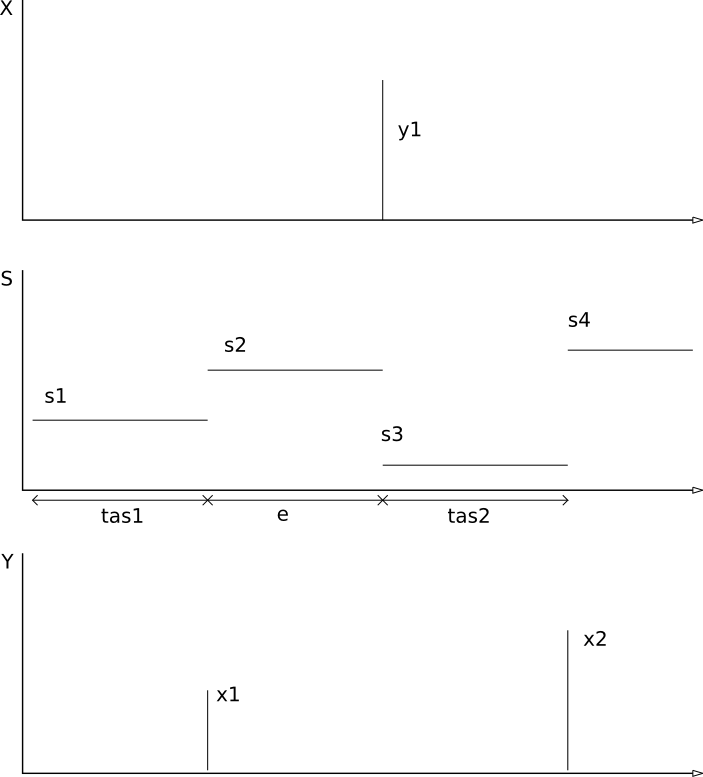
\includegraphics[scale=0.5]{devs-atomic}
	  \caption{Comportamiento de un modelo DEVS atómico}
	   \label{fig:fig2-5}
	\end{figure}

	\subsection{Acoplados}
	La descripción de un sistema puede ser completamente realizada utilizando modelos atómicos, aunque esto resulta un poco incómodo y confuso. 
	Los conjuntos de estados y las funciones de transición se vuelven inmanejables en sistemas complejos, y nunca podemos asegurar haber cubierto todos 
	los posibles estados.
	Para abordar este problema, el formalismo DEVS introduce lo que se llaman modelos acoplados, que es una forma de agrupar modelos DEVS y generar 
	nuevos modelos a partir de este agrupamiento.
	Hay dos formas de acoplamiento, la más general, en la cual se utilizan funciones de traducción entre los sub–sistemas y otra clase que adopta el 
	uso de puertos para la comunicación entre sub–sistemas. Aunque estas dos formas son equivalentes entre sí, describiremos la segunda clase, ya que 
	es la más simple y es la utilizada en el presente trabajo.
	Formalmente un modelo acoplado está representado por la octo-upla:

	\begin{equation}
	N = (X_N , Y_N , D, {M_d }, EIC, EOC, IC, Select)
	\end{equation}

	donde cada componente es:
	\begin{itemize}
	\item $X_N$ es el conjunto de eventos de entrada al modelo acoplado, representado por el producto cartesiano del conjunto de puertos de entrada $InPorts$ y
	 el conjunto de posibles valores para cada puerto. O sea un evento de entrada al modelo acoplado está representado por un par $(p, v)$ donde 
	$p \in InPorts$ y $v \in X_p$ .

	\item $Y_N$ es el conjunto de eventos que el modelo puede emitir. Es un elemento del producto cartesiano entre el conjunto de puertos de salida $OutPorts$ y
	 el conjunto de posibles valores para este puerto, o sea un evento de salida del modelo acoplado está representado por un par $(p, v)$ donde 
	$p \in OutPorts$ y $v \in Y_p$.

	\item $D$ es el conjunto de los índices a los modelos DEVS (atómicos y acoplados) que conforman este modelo. 

	\item ${M_d}$ es el conjunto de los modelos atómicos y/o acoplados (son justamente los modelos que \quotes{acopla} o \quotes{agrupa} este modelo acoplado).

	\item EIC y EOC son el conjuntos de conexiones entre los modelos internos y los puertos del modelo acoplado:
	      \begin {itemize}
		  \item EIC (o External Input Coupling) son las conexiones de entrada al acoplado, es decir, conecta un puerto de entrada del acoplado con un 
			puerto de entrada de un modelo perteneciente al acoplado.
		  \item EOC (o External Output Coupling) son las conexiones de salida del acoplado. Conecta un puerto de salida de un modelo interno del
			 acoplado con un puerto de salida del acoplado.  
	     \end{itemize}

	\item $IC$ representa las conexiones internas del modelo acoplado.

	\item Select es una función $(\mathcal{P}((D)) \to D)$ que decide qué modelo realizará primero su transición interna, si se da el caso de 
		eventos simultáneos. Es una función de \quotes{desempate} que en ciertos modelos es necesaria.
	\end{itemize}

	Formalmente:
	\begin{align*}
	EIC \in& \{((N, ip_N ), (d, ip_d )) | ip_N \in InPorts, d \in D, ip d \in InPorts_d \} \\
	EOC \in& \{((d, op_d ), (N, op_N ))  | op_N \in OutPorts, d \in D, op d \in OutPorts_d \}
	\end{align*}
	donde N es el modelo acoplado.
	\begin{equation*}
	IC \in \{((a, ip_a ), (b, ip_b )) | a, b \in D, ip a \in OutPorts_a , ip_b \in InPorts_b \}
	\end{equation*}
	donde no se permite que $a = b$.

	$InPorts$ y $Outports$ son conjuntos que describen los posibles puertos de entrada y salida respectivamente. En general se utilizan números enteros 
	para representar los puertos posibles por lo cual $InPorts = \mathbb{N}$ y $Outports = \mathbb{N}$. Los modelos acoplados son en sí mismos modelos 
	DEVS válidos; formalmente el acoplamiento (como lo definimos antes) es una operación cerrada sobre el conjunto de modelos DEVS. Acoplar modelos DEVS 
	forma nuevos modelos DEVS. Sin esta cualidad el acoplamiento resultaría inútil desde del punto de vista del formalismo. También trae muchas ventajas 
	a la hora de describir modelos DEVS y a la hora de simularlos. El acoplamiento da lugar a una estructura jerárquica de desarrollo.

	$EIC$, $EOC$ y $IC$ son conjunto de pares, de pares, como se encuentran conectados los modelos (atómicos o acoplados) a través de sus puertos con los 
	puertos de entrada, salida y con otros modelos (atómicos o acoplados) respectivamente. Tanto los puertos como los modelos son señalados por números 
	dentro de PowerDEVS, por lo que estos conjuntos estan comprendidos por elementos de la forma $(m_a, p_a), (m_b, p_b)$, donde $m_a$ y $m_b$ 
	son modelos (atómicos o no) en el actual modelo y $p_a$ y $p_b$ son sus correspondientes puertos.

	\begin{figure}[H]
	\begin{minipage}{0.5\textwidth}
	\centering
	\TBox{%
	  \TBox[]{Acoplado2 \\ \TBox{Acoplado1 \\ \TBox[]{Atómico1}\TBox{Atómico2} } \TBox{Atómico3} }}
	\end{minipage}\hfill
	\begin{minipage}{0.5\textwidth}
	\centering

	\begin{tikzpicture}[%
	  grow via three points={one child at (0.5,-0.7) and
	  two children at (0.5,-0.7) and (0.5,-1.4)},
	  edge from parent path={(\tikzparentnode.south) |- (\tikzchildnode.west)}]
	  \node {Root-Coordinator}
	    child { node {Acoplado2}		
	    child { node {Acoplado1}
	      child { node {Atómico1}}
	      child { node {Atómico2}}
	    }
	    child [missing] {}				
	    child [missing] {}				
	    child [missing] {}				
	    child { node {Atómico3}}};
	\end{tikzpicture}
	\end{minipage}

	\caption{Ejemplo de un modelo jerárquico.}

	\end{figure}


	\subsection{Modelos DEVS parametrizados}
	Definiremos primero los modelos DEVS parametrizados\cite{BKC12} como un paso previo hacia el formalismo DEVS vectorial (Vectorial DEVS o VECDEVS), 
	el cual es una herramienta que nos facilitará representar modelos de gran escala en forma gráfica, en particular este formalismo se encuentra implementado 
	en la herramienta PowerDEVS.

	Formalmente : dado un modelo DEVS atómico $M$ obtenemos un Modelo DEVS Parametrizado:
	\begin{equation}
	M (p) = \{X, Y, S, \delta_{int}, \delta_{ext} ,\lambda , ta, p\}
	\end{equation}

	donde $p \in P$ es un parámetro que pertenece a un conjunto de parámetros arbitrario tal que $\delta_{int}$ , $\delta_{ext}$ , $\lambda$ y $ta$ 
	dependen también de $p$.
	Notar que dos modelos DEVS $M (p_1 )$, $M (p_2 )$ con $p_1 \neq p_2$ pueden exhibir distintos comportamientos aunque compartan los mismos conjuntos 
	de entrada, salida y de estados ($X$, $Y$ , y $S$, respectivamente).

	\subsection{Modelos Vectoriales}
	Dado el modelo escalar DEVS Parametrizado:
	\begin{equation}
		M (p) = \{X, Y, S, \lambda_{int} , \lambda_{ext} , \lambda, ta, p\}
		\end{equation}

		definimos un modelo Vectorial DEVS\cite{BKC12} como la estructura:
		\begin{equation}
		V_D = \{N, X_V, Y_V, P, \{M_i\}\},
		\end{equation}
		donde:
		\begin{itemize}
		\item $N \in \mathbb{N}$ es la dimensión del modelo vectorial.

		\item $X_V = X \times Index \bigcup \{-1\}$ es el conjunto de eventos de entradas vectorial donde $X$ es el conjunto de eventos de entrada del modelo 
		escalar e $Index = {1, \ldots , N }$ es el conjunto de índices que indican cuál de los modelos DEVS atómicos recibirá el evento.

		\item $Y_V = Y \times Index$ es el conjunto de eventos de salida vectorial donde $Y$ es el conjunto de eventos de salida del modelo escalar e 
		$Index = {1, \ldots , N }$ es el conjunto de índices que indica que modelo escalar de los $N$ , emitió el evento. 

		\item $P$ es un conjunto de parámetros arbitrario.

		\item Para cada índice $i \in Index$, $p(i) \in P$ es un parámetro y $M_i = M (p(i))$ es el modelo DEVS Parametrizado escalar.
	\end{itemize}

	\subsubsection{Interfaz entre DEVS Vectorial y DEVS}
	Para conectar bloques vectoriales y bloques escalares es necesarios bloques que hagan de interfaz entre los dos formalismo, además, introducimos 
	un bloque necesario para realizar modelos más complejos y conectar los diferentes componentes de un modelo vectorial entre sí.

	\begin{itemize}
		\item Escalar a Vector (Scalar to Vector): Este bloque simplemente agrega al indice $i$ al evento escalar que recibe, transformándolo en un 
			evento vectorial. Este modelo también posee un comportamiento especial para enviar el mismo evento en todas las componentes vectorial 
			al mismo tiempo, cuando $i = -1$, cada evento de entrada es trasmitido para todas las componentes del vector salida.
		\item Vector a escalar (Vector to Scalar): Este bloque tiene un parámetro $i$ que contiene el índice del vector de eventos a retransmitir, 
			cuando recibe un evento con indice $j=i$, remueve el indice y retransmite el evento escalar.
		\item Index Shift: El modelo más simple es el Index Shift. Cuando se recibe un evento con el valor $(x,i)$, emite un evento de salida $(x, i+sh)$, 
			donde $sh$ es un parámetro entero.
	\end{itemize}

	Es importante ver que los mensajes entre bloques vectoriales es un par donde uno de sus componentes es un número natural, que funciona como índice,
	el cual nos permite determinar en que posición del vector se encuentra la otra componente.

	En este trabajo todos estos bloques se la ha agregado la dimensión $N$ como parámetro, esto es necesario para realizar la conversión de los modelos,
	 de forma que no existan desconexiones a nivel Modelica, lo cual se reflejaría en un modelo con menos ecuaciones que variables, es decir un modelo 
	no balanceado.
	 
\section{PowerDEVS}
	PowerDEVS\cite{BK11}  es un programa, concebido para ser utilizado por expertos programadores DEVS, así como usuarios finales que solo quieren 
	conectar bloques y simular.

	\begin{figure}[!htbp]
	  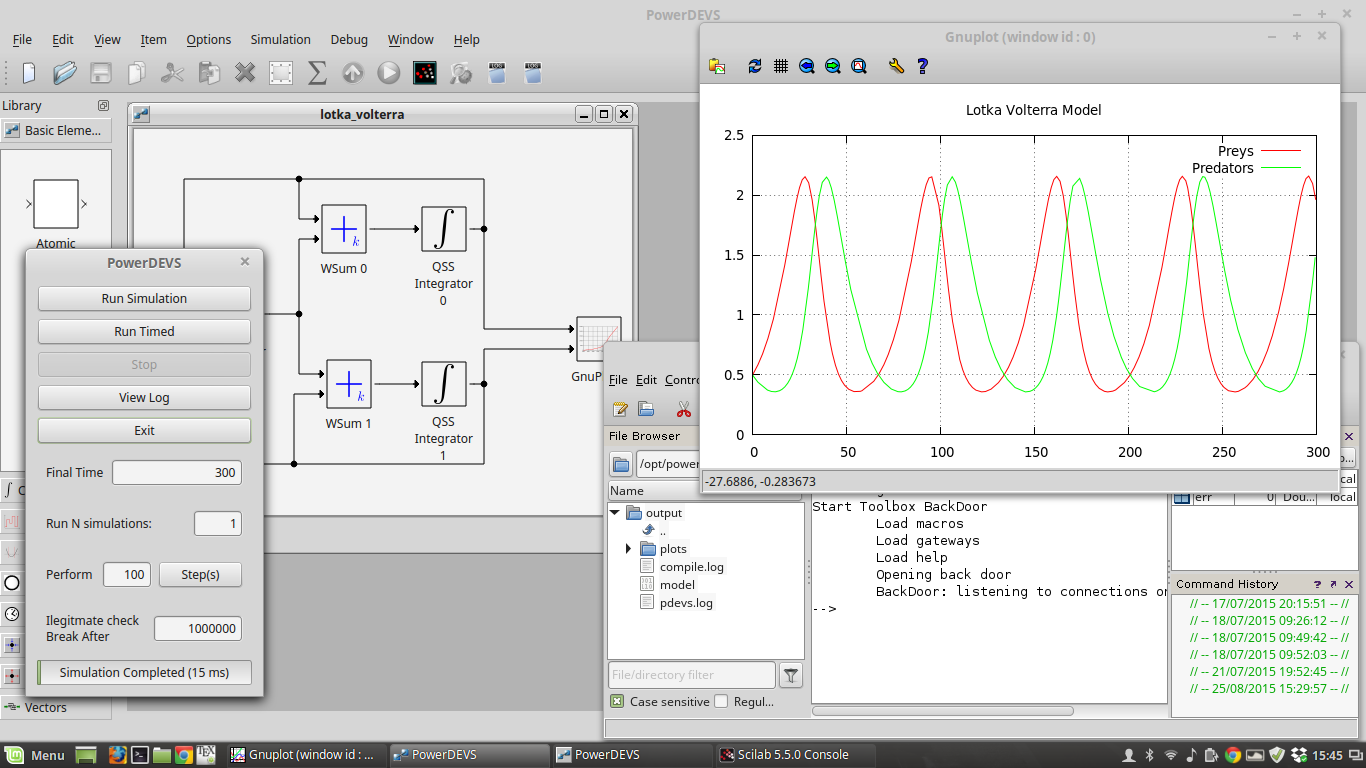
\includegraphics[width=\textwidth]{powerdevs}
	  \caption{Interfaz gráfica de PowerDEVS}
	   \label{fig:powerdevsgui}
	\end{figure}

	PowerDEVS esta compuesto por varios programas independientes:
	\begin{itemize}
		\item El \emph{editor de modelos}, es desde el punto de vista del usuario, el principal programa de PowerDEVS, pues provee la interfaz gráfica 
			y enlaces para las demás aplicaciones. 
		Además de construir, manejar modelos y librerías, permite lanzar las simulaciones (lanzando el \emph{Pre procesador}) y editar los bloques 
		elementales hasta su definición atómica de modelo (invocando el \emph{Editor Atómico}).
		La ventana principal de \emph{Editor de Modelo} permite al usuario crear y abrir modelos y librerías. También permite a las librerías ser 
		exploradas y los bloques arrastrados de las librerías a los modelos.
		La ventana del Modelo provee todas las funcionalidades típicas para la edición gráfica para poder copiar, cambiar el tamaño, rotar, etc. mientras 
		que las conexiones pueden ser dibujadas entre los diferentes puertos.
		La ventana de Edición de Bloques, nos permite configurar la apariencia gráfica y elegir los parámetros del bloque y, en el caso de los modelos 
		atómicos, seleccionar el archivo que contiene el código asociado con la definición DEVS.

		\item El \emph{Editor de Modelos Atómicos} facilita la edición del código C++ correspondiente a cada modelo atómico DEVS, el usuario debe 
		definir las variables que forman el estado y parámetros y 6 funciones en sus correspondientes solapas, Init, Time Advance, Internal transition, 
		External transition, Output y Exit  
		Cuando el modelo se guarda, el código es guardado en los archivos .cpp y .h. 

		\item El \emph{Pre procesador}, toma un archivo .pdm (o .pds) producido por el \emph{Editor de Modelos} y produce el programa que corre 
		la simulación. Básicamente traduce el archivo .pdm a un archivo de cabecera .h que enlaza el simulador y el coordinador de acuerdo a la 
		estructura del modelo pasando además los parámetros definidos para el modelo.
		El \emph{Pre procesador}, además produce un Makefile (Makefile.include) el cual invoca el compilador para generar el programa que implementa 
		la simulación.

		\item La \emph{interfaz de simulación}, que corre el programa que implementa la simulación y permite variar parámetros de la simulación 
		como tiempo final, números de simulación a ejecutar, y el modo de simulación (normal, cronometrada, pasa o paso, etc.).

		\item Una instancia de Scilab, que actúa como un espacio de trabajo, donde los parámetros pueden ser leídos, y los resultados pueden ser exportados.
	\end{itemize}


	En la figura \ref{fig:lk-powerdevs} se puede ver el modelo Lotka Volterra que acompaña la instalación de PowerDEVS, este modelo (aunque no visible en la figura)
	tiene valores iguales a los expresados en el modelo equivalente anteriormente presentado en el listado \ref{lst:LotkaVolterra.mo}. 
	las dos conexiones contra el bloque \texttt{GnuPlot 0} representando las variables \texttt{x} e \texttt{y} es decir presa y depredadores, ambas variables 
	son el resultado de la integración por lo que los integradores \texttt{QSS Integrato 0} y \texttt{QSS Integrato 1} contienen en sus puerto de entrada los 
	valores \texttt{dx/dt} y \texttt{dy/dt}. 
	Los bloques \texttt{WSum 0} y \texttt{WSum 1}, tiene constante de forma que el valor de salida (\texttt{y}) queda definido como
	$y = K[0] * u0 + K[1] * u1 + \dots + K[7] * u7$ y en nuestro modelo son $K[0] = 0.1$ y $K[1] = -0.1$ en ambos bloques \texttt{WSum 0} y \texttt{WSum 1}.
	Replicando nuestra la ecuación de nuestro modelo.
	

	\begin{figure}[!htbp]
	  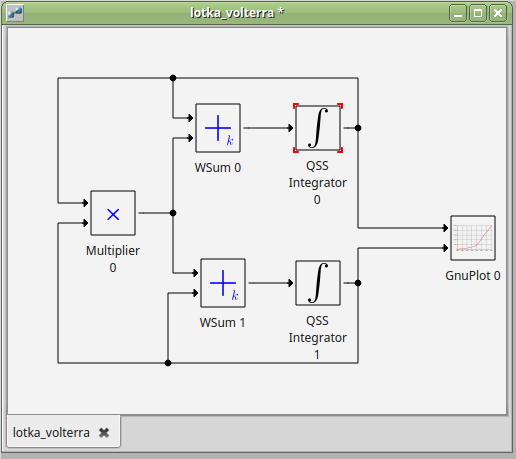
\includegraphics[width=\textwidth]{lk-powerdevs}
	  \caption{Modelo Lotka Volterra descripto en PowerDEVS}
	   \label{fig:lk-powerdevs}
	\end{figure}



\chapter{Conversión de modelos DEVS}
En este capitulo describimos en detalles los pasos para realizar la transformación, utilizaremos el modelo ya presentado e introduciremos un modelo PowerDEVS con componentes vectoriales con el fin de ilustrar la transformación de estos componentes.

\section{Modelos DEVS}

        \subsection{Archivos PDS}
        PowerDEVS trabaja principalmente con dos archivos, .PDM y .PDS.
        Los archivos PDM es utilizado por el editor de modelos, pues contiene información estructural, así como información de posición de los modelos dentro del 
        editor, sus parámetros, lo cual indica nombre, tipo y valor, descripción de los modelos, la cantidad de puertos de cada modelo y las conexiones
        entre los modelos, los detalles de como esas conexiones son visualizadas por lineas y los detalles del recorrido de esas lineas. 
        Todos estos elementos son utilizados en primera medida con el editor de modelos, pero tambien son utilizados para generar el archivo PDS el cual es el 
        genera el código de la simulación.
        El archivo PDS contiene información estructural del modelo necesaria para realizar la simulación, en el listado \ref{lst:pdsstruc} se pueden ver un 
        esbozo de su estructura.
        
\begin{listing}[H]
\begin{minted}{console}
Root-Coordinator
 {
  Simulator
   {
        ...
   }
   ...
    Coordinator
     {
      ...
     }
   ...     
  Simulator
   {
        ...
   }
  EIC
   {
   }
  EOC
   {
   }
  IC
   {
        ...
   }
 }
\end{minted}
\caption{Estructura de un archivo PDS.}
\label{lst:pdsstruc}
\end{listing}

        Se puede observar un \texttt{Root-Coordinator} el cual contiene (marcado entre llaves) una lista de \texttt{Simulator} que representan los modelos atómicos
        y/o \texttt{Coordinator} que representan los modelos acoplados y tres listas de 
        conexiones \texttt{EIC}, \texttt{EOC} y \texttt{IC}, conexiones de entrada externa (External Input Connections), 
        conexiones de salida externa (external output connections) y conexiones internas (Internal Connections).

        Los modelos acoplados dado que también son modelos DEVS, replican la estructura listado \ref{lst:pdsstruc}.


        Para poder leer esta estructura se cuenta con la librería de PowerDEVS\footnote{http://sourceforge.net/p/powerdevs/code/HEAD/tree/} la cual nos permite acceder
        a la estructura desde C++. 


\section{Modelos Atómicos}
Los modelos atómicos no son traducidos automáticamente, deben ser provistos siguiendo la siguiente especificación:

\begin{itemize}
\item El código debe ser Modelica ($\mu$modelica) valido y estar ubicado en el mismo directorio (y nombre del archivo) del código C que el modelo atómico PowerDEVS, con el mismo nombre que el archivo .h, pero con extensión .mo
\item Los parámetros del modelo DEVS deben ser pasado en el parámetro $p$
\item Los valores de entrada del modelo son asociados a la variable $u$
\item Los valores de salida del modelos son asociados a la variable $y$
% \item La cantidad de ecuaciones y variables debe ser igual.
\end{itemize}

Por ejemplo el código del integrador, originalmente ubicado en el archivo qss\_integrator.h de PowerDEVS, se ubica en el archivo qss\_integrator.mo ambos dentro del directorio qss.

\begin{minted}{modelica}
class QSSIntegrator
  parameter Real p[4]={0,0,0,0};
  parameter Real x0 = p[4];
  Real u[1];
  Real y[1](start = {x0});
equation
  der(y[1]) = u[1];
end QSSIntegrator;
\end{minted}

Los parámetros son remplazadas en el modelo, evaluados en Scilab, lo que los transforma en float, los cuales son presentados como reales (Real) en el código.

Los modelos no encontrados son ignorados en la traducción.

\section{Modelos Acoplados Planos}

Llamamos \emph{Modelos Acoplados Planos} a los Modelos Acoplados que solo contienen \emph{Modelos Atómicos}. Estos modelos son convertidos en modelos Modelica de la siguiente forma:
Para el $i$-esimo modelo atómico del modelo acoplado
\begin{itemize}
        \item Se incluye el código Modelica del $i$-esimo modelo atómico
        \item Se remplazan los parámetros $p$ por los del $i$-esimo modelo atómico.
        \item Se reescriben todas las variables (excepto la variable $time$) construido con $i$ y el nombre del modelo (en Modelica).
\end{itemize}

Luego cada conexión entre Modelos Atómicos es replicada en el código de Modelica resultante. Los modelos Atómicos cuyo entrada (o salida) son escalares son conectados con un ecuación del tipo $u = y$ mientras que los modelos vectoriales son conectados con la misma ecuación, solo que dentro de un $for$.

Veamos como se realiza la transformación paso a paso con un ejemplo de un integrador.

\begin{figure}[!htbp]
\begin{center}
  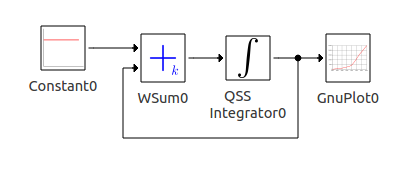
\includegraphics[scale=0.5]{integrator-devs}
  \caption{DEVS Ejemplo de Integrador}
  \end{center}
   \label{fig:integrator}
\end{figure}

Este modelo incluye los siguientes modelos atómicos:
\begin{itemize}
        \item Constante: Constant0
\begin{minted}{modelica}        
class Constant
  parameter Real k = 1;
  Real y[1];
equation
  y[1] = k;
end Constant;
\end{minted}

        \item Sumador: WSum0
\begin{minted}{modelica}        
class WSum
  parameter Real p[9]={0,0,0,0,0,0,0,0};
  parameter Integer n= integer(p[9]);
  parameter Real w[n] = p[1:n];
  Real u[n];
  Real y[1];
equation
  y[1]=u*w;
end WSum;
\end{minted}

        \item Integrador: QSSIntegrator0
\begin{minted}{modelica}        
class QSSIntegrator
  parameter Real p[4]={0,0,0,0,0,0,0,0};
  parameter Real x0 = p[4];
  Real u[1];
  Real y[1](start = {x0});
equation
  der(y[1]) = u[1];
end QSSIntegrator;
\end{minted}

        \item Gnu Plot : GNUPlot0, el cual no va a ser convertido debido a que no tiene un modelo equivalente en modelica.
\end{itemize}

El integrador es el primero en la lista de atómicos dentro del PowerDEVS, por lo que es el primero en procesarse y por lo tanto obtiene el prefijo $<nombre modelo>\_0\_$ para sus variables, también remplazamos los parámetros provenientes de la simulación de PowerDEVS:

\begin{minted}{modelica}        
class QSSIntegrator
  parameter Real QSSIntegrator_0_p[4]={0,1e-06,0.001,0};
  parameter Real QSSIntegrator_0_x0 = 0;
  Real QSSIntegrator_0_u[1];
  Real QSSIntegrator_0_y[1](start = {QSSIntegrator_0_x0});
equation
  der(y[1]) = QSSIntegrator_0_u[1];
end QSSIntegrator;
\end{minted}

\begin{minted}{modelica}
class WSum
  parameter Real WSum_1_p[9]={1,(-1),0,0,0,0,0,0,2};
  parameter Integer WSum_1_n= integer(2);
  parameter Real WSum_1_w[WSum_1_n] = p[1:WSum_1_n];
  Real WSum_1_u[WSum_1_n];
  Real WSum_1_y[1];
equation
  WSum_1_y[1]=WSum_1_u*WSum_1_w;
end WSum;
\end{minted}

\begin{minted}{modelica}        
class Constant
  parameter Real Constant_2_k = 1;
  Real Constant_2_y[1];
equation
  Constant_2_y[1] = Constant_2_k;
end Constant;   
\end{minted}

En este punto podemos juntar las declaraciones y ecuaciones dentro de un nuevo modelo, el cual llamaremos con el nombre del modelo a convertir.

\begin{minted}{modelica}        
class Integrador
  parameter Real QSSIntegrator_0_p[4]={0,1e-06,0.001,0};
  parameter Real QSSIntegrator_0_x0 = 0;
  Real QSSIntegrator_0_u[1];
  Real QSSIntegrator_0_y[1](start = {QSSIntegrator_0_x0});
  parameter Real WSum_1_p[9]={1,(-1),0,0,0,0,0,0,2};
  parameter Integer WSum_1_n= integer(2);
  parameter Real WSum_1_w[WSum_1_n] = p[1:WSum_1_n];
  Real WSum_1_u[WSum_1_n];
  Real WSum_1_y[1];
equation
  der(y[1]) = QSSIntegrator_0_u[1];
  WSum_1_y[1]=WSum_1_u*WSum_1_w;
  Constant_2_y[1] = Constant_2_k;
end QSSIntegrator;
\end{minted}

Luego de agregar las equaciones correspondientes a las interconecciones de los modelos atómicos, obtenemos el siguiente modelo
        
\begin{minted}{modelica}
model Integrador
  parameter Real QSSIntegrator_0_p[4] = {0,1e-06,0.001,0};
  parameter Real QSSIntegrator_0_x0 = 0;
  Real QSSIntegrator_0_u[1];
  Real QSSIntegrator_0_y[1](start = {0});
  parameter Real WSum_1_p[9] = {1,(-1),0,0,0,0,0,0,2};
  parameter Integer WSum_1_n = integer(2);
  parameter Real WSum_1_w[WSum_1_n] = WSum_1_p[1:WSum_1_n];
  Real WSum_1_u[WSum_1_n];
  Real WSum_1_y[1];
  parameter Real Constant_2_k = 1;
  Real Constant_2_y[1];
  equation
    der(QSSIntegrator_0_y[1]) = QSSIntegrator_0_u[1];
    WSum_1_y[1] = WSum_1_u*WSum_1_w;
    Constant_2_y[1] = 1;
    QSSIntegrator_0_u[1] = WSum_1_y[1];
    WSum_1_u[2] = QSSIntegrator_0_y[1];
    WSum_1_u[1] = Constant_2_y[1];
end Integrador;
\end{minted}

\section{Modelos Acoplados Jerárquicos}
En la sección anterior mostramos como son convertidos modelos acoplados compuestos por modelos atómicos, para convertir un modelo acoplado jerárquico, es decir con más modelos acoplados internos, vamos a generar un modelo acoplado plano, equivalente al modelo jerárquico inicial.

Para realizar el aplanado, se recorre recursivamente los modelos acoplados:

\begin{itemize}
\item por cada modelo acoplado si solo tiene modelos atómicos, es remplazado por los modelos atómicos internos, los cuales se encuentran conectados sin modificaciones excepto por las conexiones externas, las cuales son reasignadas de forma de mantener las conexiones.
\item si el modelo acoplado contiene otros modelos acoplados entonces aplanamos ese modelo recursivamente.
\end{itemize} 

De esta forma obtenemos un modelo con solo modelos atómicos el cual podemos convertir con el procedimiento anterior.

A modo de ejemplo se muestran, el esquema del integrador de la sección anterior con un modelo acoplado en \ref{fig:acomplado} y luego el mismo modelo en \ref{fig:aplanado}, aplanado, el cual puede ser convertido pues ya no presenta jerarquias.

\begin{figure}[H]
\centering
 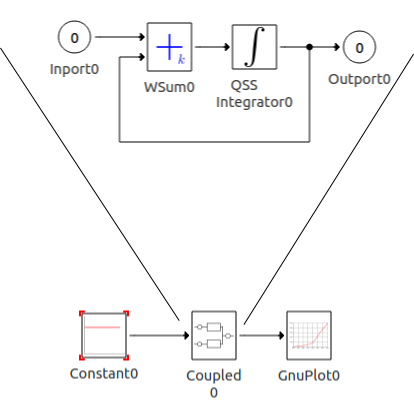
\includegraphics[width=0.5\linewidth]{integrator-sample}
 \caption{Representación de un modelo simple de integrador acoplado}
 \label{fig:acomplado}
\end{figure}


\begin{figure}[H]
\centering
 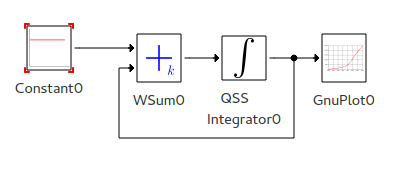
\includegraphics[width=0.5\linewidth]{integrator-expanded}
 \caption{Representación del modelo de integrador aplanado }
 \label{fig:aplanado}
\end{figure}



\section{Modelos Vectoriales}
Los modelos vectoriales difieren levemente de los atómicos no vectoriales. Estos modelos pueden tener tanto la entrada como la salida de sus conectores de forma vectorial, por lo que los modelos vectoriales deben indicarlos con la anotación de Modelica $PD2MO$, por ejemplo:
\begin{itemize}
\item $annotation(PD2MO = {Scalar, Vector});$ cuando la entrada es escalar, es decir no vectorial y la salida vectorial
\item $annotation(PD2MO = {Vector, Scalar});$ cuando la entrada es vectorial y la salida vectorial
\item $annotation(PD2MO = {Vector, Vector});$ cuando ambos, la entrada y salida son vectoriales.
\item $annotation(PD2MO = {Scalar, Scalar});$ cuando ambas entrada y salida son escalares, este es el caso por omisión y no es necesario declararlo.
\end{itemize}

Además las variables de entradas $u$ y salidas $y$ vectoriales deben ser definidas como vectores en Modelica. A modo de ejemplo se muestra a continuación el archivo vector/qss\_integrator\_vec.mo. Este modelo atómico representa $N$ integradores y es la version vectorial del integrador atómico mostrado antes.

\begin{minted}{modelica}
class VecInt
  parameter Real p[5] = {0, 10, 0, 0, 10};
  constant Integer N = p[5];
  parameter Real x0 = p[4];
  Real u[N, 1];
  Real y[N, 1];
initial algorithm
  for i in 1:N loop
    y[i, 1] := x0;
  end for;
equation
  for i in 1:N loop
    der(y[i, 1]) = u[i, 1];
  end for;
  annotation(PD2MO = {Vector, Vector});
end VecInt;
\end{minted}


\section{Equivalencia semántica de la conversión}
Hay tres situaciones que debemos considera al momento de verificar la equivalencia semántica
\begin{itemize}
\item Modelos Atómicos : Los modelos atómicos son convertidos por el usuario, los que se han propuesto en el código mantienen una conservación de la semántica que no es estricta y se trató manualmente. 
\item Modelos Acoplado - Plano : Como fue descripto en la sección Modelos Acoplados Planos, los modelos son conectados por una ecuación en caso de ser un modelo escalar, o por un conjunto de ecuaciones (expresadas en una sentencia $for$). En este caso esta conversión (conexión por igualdad) no mantiene la semántica, pues la semántica de una conexión (o grupo de conexiones en el caso vectorial) es diferente de la semántica de un ecuación (o grupos de ecuaciones).

\item Modelo Jerárquico : En este caso si podemos probar la equivalencia semántica, entre el modelo original, es decir un modelo acoplado que incluye más modelos acoplados, con un modelo \quotes{aplanado} (solo con modelos atómicos). Esto se debe a que el formalismo DEVS es cerrado bajo el acoplamiento \cite{Zeigler:2000:TMS:580780} y \cite{zeigler1984multifacetted}, lo que permite remplazar un modelos acoplado por equivalentes atómicos, conectados apropiadamente.
\end{itemize}


\chapter{Detalles de la implementación}
	A continuación se presenta el pseudo código que implementa las transformaciones descriptas en este trabajo, 
	el código completo puede encontrarse en \url{https://github.com/lucciano/pd2mo}, el cual utiliza dos librerias, Modelica C Compiler 
	\footnote{http://sourceforge.net/projects/modelicacc/} el cual nos permite manipular la estructura de los modelos y evaluar los parámetros.
y libreria de PowerDEVS \footnote{http://sourceforge.net/projects/powerdevs/} para leer los archivos PDS.

El programa esta separado en 4 módulos:

\section{Programa Principal}

El Programa principal en el archivo main.cpp, el cual es responsable de la interfaz con el usuario (linea de comando) y lanzar la transformación de la simulación, asi como establecer los archivos desde donde se lee y hacia donde se escriben la simulación de powerDEVS y Modelica, respectivamente.


\begin{algorithm}[H]
\begin{algorithmic}[1]
\State modelCoupled *cm $\gets$ parsePDS(QString::fromStdString(src\_infile));
\State modelCoupled *qm $\gets$ flatter::flat(cm);
\State Pd2Mo q $\gets$ Pd2Mo();
\State q.transform(flatted, modelname, \&outfile, \&oFlogfile);
\State AST\_StoredDefinition sd $\gets$ parseFile(src\_outfile.c\_str(),\&amp;r);
\State mda *m $\gets$ new mda();
\State If *i $\gets$ new If();
\State outfile $\ll$ m$\rightarrow$\Call{visitClass} 
		{prod$\rightarrow$visitClass( i$\rightarrow$visitClass( 
			*sd$\rightarrow$models()$\rightarrow$begin()))} $\ll$ endl;

\end{algorithmic}
\caption{main(src\_infile)}
\end{algorithm}

\section{Transformación Principal}
La clase \emph{Pd2Mo} implementa las principales partes de la transformación, la cual incluye abrir el archivo PDS, e invocar el aplanado, obtener los diferentes modelos modelica que representan los modelos atómico, prevenir la colisión de nombres, crear el modelo final y realizar las conexiones.

\begin{algorithm}[H]
\begin{algorithmic}[1]
\State modelCoupled *model $\gets$ parsePDS(qfilename);
\State AST\_ClassList classList $\gets$ getAsClassList(model); 
\State int j $\gets$ 0\;
\For{class en classList}
 	\If{La clase esta traducida a $\mu$Modelica}

 		\State Prefijamos las variables con el nombre del modelo $class$ y la posición $j$ que ocupan en la lista;
 		\State Remplazamos la entrada $class$ dentro de la lista por su copia producida en el paso anterior;
 	\EndIf
\EndFor
\State Creamos un modelo $modeloMo$;
\For{class en classList}
 	\State Combinamos el modelo $class$ con el $modeloMo$;
\EndFor

\For{ic en Conexión Interna del Modelo}
	\State Las conexiones ic estan definidas como dos pares de números, cada par señalan número  de modelo y número de puerto, en este caso los puertos deben ser desfasados en uno, pues los puertos en nuestra representación son los sub-indices de $u$ e $y$ para cada modelo, pero el primer elemento de los arreglos en Modelica comienzan.
  	\If{los modelos de ic son Escalares}
  		\State Se agrega la ecuación que representa la conexión entre los modelos;
  	\ElsIf{los modelos de ic son Vectoriales}
  		\State Se agregan $N$ ecuaciones indexadas por $i$ que representa la conexión, vectorial entre los modelos mediante una sentencia \texttt{For};
  	\Else
  		\State No se conoce la conexión;
	\EndIf
\EndFor
\end{algorithmic}
 \caption{Pd2Mo::transform()}
\end{algorithm}

\section{Aplanado de modelos acoplados}
La clase \emph{flatter} implementa el aplanado de los modelos acoplados descripto en la sección \ref{aplanado}.
 
\begin{algorithm}[H]
\begin{algorithmic}[1]
\For{ModeloHijo en Lista de Modelos}
  	\If{Tipo de ModeloHijo es COUPLED}
  		\For{ModeloHijo2 en Lista de ModeloHijo$\rightarrow$ModeloHijo}
  			 	\If{Tipo de ModeloHijo2 es ATOMIC}
  			 		\State Copiamos el ModeloHijo2 al ModeloResultado;
				\Else
  			 		\State Copiamos el aplanado de ModeloHijo2;
				\EndIf
  			 	\For{Conexión del Modelo}
  			 		\If{Si la conexión involucra un modelo \quotes{aun no procesado}}
  			 			\State Las conexiones deben ser modificadas teniendo en cuenta los modelos agregados en el aplanado;
					\EndIf
  			 		\If{Si la conexión involucra como destino el modelo acoplado ModeloHijo}
  			 			\State Se crea una nueva conexión (en ModeloResultado) entre los modelos agregado recientemente según la conexión del puerto de entrada del ModeloHijo y el origen de la conexión;
  			 			\State La conexión se marca para ser borrada;
					\EndIf
  			 		\If{Si la conexión involucra como origen el modelo acoplado ModeloHijo}
  			 			\State Se crea una nueva conexión (en ModeloResultado) entre los modelos agregado recientemente según la conexión del puerto de salida del ModeloHijo y el destino de la conexión;
  			 			\State La conexión se marca para ser borrada;
					\EndIf
  			 		\If{Si la conexión fue marcada}
						
						\State Se borra la conexión
					\EndIf
				\EndFor
		\EndFor
  	\Else

  		\State Copiamos el nodo ModeloHijo al ModeloResultado 
  		\State Copiamos las conexiones del ModeloHijo y cualquier otro ModeloHijo que ya haya sido procesado

	\EndIf
\EndFor
\Return ModeloResultado
\end{algorithmic}
\caption{flatter::flat}
\end{algorithm}

 
\section{Transformaciones para $\mu$-Modelica} \label{sec:transform}
	Tanto la clase \texttt{mda}, \texttt{prodint} y \texttt{If} son implementadas con el patron de diseño de visitadores sobre 
	el árbol sintáctico abstracto\footnote{un árbol de sintaxis abstracta (AST), o simplemente un árbol de sintaxis, es una representación 
	de árbol de la estructura sintáctica abstracta (simplificada) del código fuente escrito en cierto lenguaje de programación.}, por lo que 
	cada clase es implementada heredando de una clase común (Traverser), la cual retorna una copia del AST y remplaza una parte este según sea el 
	objetivo de la clase.
	
	Estas transformaciones son necesarias dado que al momento de realizar este trabajo no son soportadas por el QSS-Solver, ya que no son $\mu$-Modelica
	valido.
	Arreglos multidimensionales no están soportados dado que no es $\mu$-Modelica valido, ya que los arreglos son de una sola dimensión, mientras que el producto 
	vectorial de dos vectores no estaba implementado en un principio, ya se encuentra implementado en una versión de desarrollo, y la transformación \texttt{If}
	fue implementada para simplificar le código final.
	 
	  \begin{itemize}
		\item  \texttt{mda}: Remplaza expresiones de la forma \texttt{X[N,k]}, donde $k \in \mathbb{N}$ o evalúa a una variable que evalúa a una expresión 
			$\in \mathbb{N}$, es remplazado por \texttt{X\_k[N]}.

\begin{figure}[htp]
\centering
\begin{cminted}{modelica}
Real IndexShift_2_u[IndexShift_2_N,1];
\end{cminted}

$\Downarrow$

\begin{cminted}{modelica}
Real IndexShift_2_u_1[IndexShift_2_N];
\end{cminted}
\end{figure}


		\item $prodint$: Remplaza expresiones de la forma $u[i, 1:nin] * w$ por expresiones de la forma 
			u[i,1] * w[1] + u[i,2] * w[2] .... + u[i,nin] * w[nin], donde $nin \in \mathbb{N}$ o evaluá a una variable que evaluá a una 
			expresión $\in \mathbb{N}$

\begin{figure}[htp]
\centering
\begin{minted}{modelica}
    VectorSum_3_y_1[VectorSum_3_i] = 
	VectorSum_3_u[VectorSum_3_i, 1:VectorSum_3_nin] * VectorSum_3_w;
\end{minted}

(Donde \texttt{VectorSum\_3\_nin = 4}  y \texttt{VectorSum\_3\_w} tiene dimensión 4, lo que es necesario para que quede definida el producto de dos vectores en modelica.)

$\Downarrow$

\begin{minted}{modelica}
    VectorSum_3_y[1,VectorSum_3_i] = 
	VectorSum_3_u[1,VectorSum_3_i]*VectorSum_3_w[1]+
	VectorSum_3_u[2,VectorSum_3_i]*VectorSum_3_w[2]+
	VectorSum_3_u[3,VectorSum_3_i]*VectorSum_3_w[3]+
	VectorSum_3_u[4,VectorSum_3_i]*VectorSum_3_w[4];
\end{minted}
\end{figure}

		\item $If$: Remplaza expresiones de la forma $if(v){eq_1}else{eq_2}$ si $v$ evaluá a un booleano (a partir de parámetros o constantes, 
			es decir en análisis estático) se remplaza por $eq_1$ o $eq_2$ si es $v$ es verdadero o falso respectivamente.

\begin{figure}[htp]
\centering
\begin{minted}{modelica}
  if IndexShift_2_Shift > 0 then
    for IndexShift_2_i in 1:IndexShift_2_N-IndexShift_2_Shift loop
      IndexShift_2_y_1[IndexShift_2_i+IndexShift_2_Shift] = 
	IndexShift_2_u_1[IndexShift_2_i];
    end for;
    for IndexShift_2_i in 1:IndexShift_2_Shift loop
      IndexShift_2_y_1[IndexShift_2_i] = 0;
    end for;
  else
    for IndexShift_2_i in 1:IndexShift_2_N-IndexShift_2_Shift loop
      IndexShift_2_y_1[IndexShift_2_i] = 
		IndexShift_2_u_1[IndexShift_2_i - +IndexShift_2_Shift];
    end for;
    for IndexShift_2_i in IndexShift_2_N + IndexShift_2_Shift : IndexShift_2_N loop
      IndexShift_2_y_1[IndexShift_2_i] = 0;
    end for;
  end if;
\end{minted}

(Con \texttt{Shift $> 0$})

$\Downarrow$

\begin{minted}{modelica}
  for IndexShift_2_i in 1:IndexShift_2_N-IndexShift_2_Shift loop
    IndexShift_2_y_1[IndexShift_2_i+IndexShift_2_Shift] = 
	IndexShift_2_u_1[IndexShift_2_i];
  end for;
  for IndexShift_2_i in 1:IndexShift_2_Shift loop
    IndexShift_2_y_1[IndexShift_2_i] = 0;
  end for;
\end{minted}
\end{figure}
	  \end{itemize}


\chapter{Ejemplos y Resultados}
	En este capitulo mostramos los resultados del presente trabajo, comparamos los resultados de la ejecución de 5 modelos, los tiempos de ejecución y 
		comparamos los resultados obtenidos. Los modelos ejecutados tanto los originales, en PowerDEVS, y los modelos transformados en 
		$\mu$-Modelilca se encuentran en \url{https://github.com/lucciano/pd2mo/tree/master/doc/tesina/src}


\section{Comparación de performance}
	A continuación por cada uno de los modelos se muestra su modelo en Powerdevs seguido de una gráfica de valores en tiempo de las simulaciones, 
	a la izquierda se muestra el resultado en PowerDEVS y a la derecha los de QSS-Solver convertidos por la herramienta desarrollada.

\section{Líneas de Transmisión}
	El siguiente sistema de ecuaciones representan un modelo a parámetros concentrados de una línea de transmisión formada por $N$ secciones de circuitos LC:

\begin{equation*}
\begin{split}
\dot{v}_{j} &= \frac{i_{j} - i_{j+1}}{C} \\
\dot{i}_{j} &= \frac{v_{j-1} - v_{j}}{L} \\	
\end{split}
\end{equation*}

para $j = 1 \dots N$

Consideramos también un pulso de entrada:
\begin{equation}
v_0(t) = \left\{ 
  \begin{array}{l l}
    1 \text{ si } t < 1 \\
    0 \text{ en caso contrario }
  \end{array} \right.
\end{equation}

 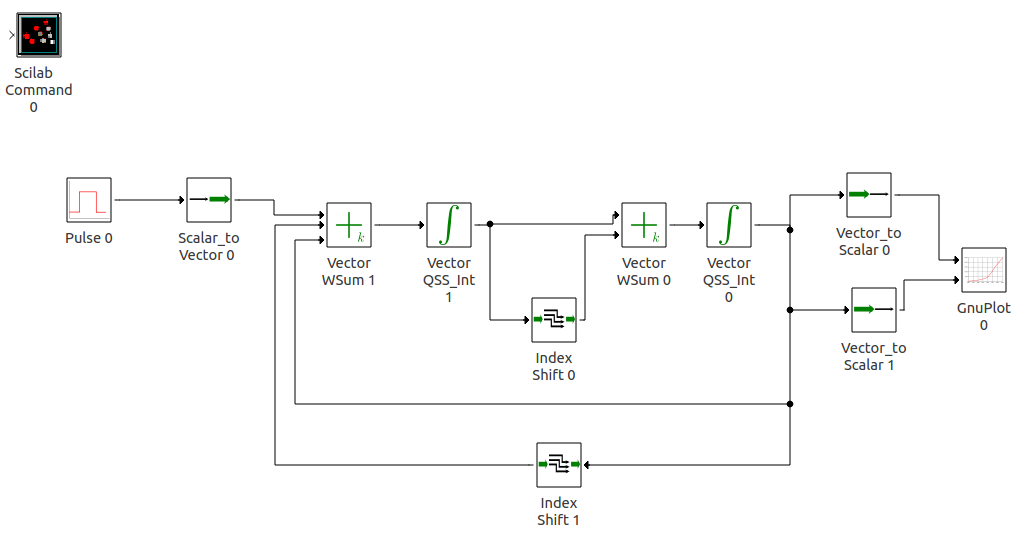
\includegraphics[width=0.75\linewidth]{lclines}

\begin{figure}[H]
\centering
\begin{minipage}{0.5\textwidth}
\centering
 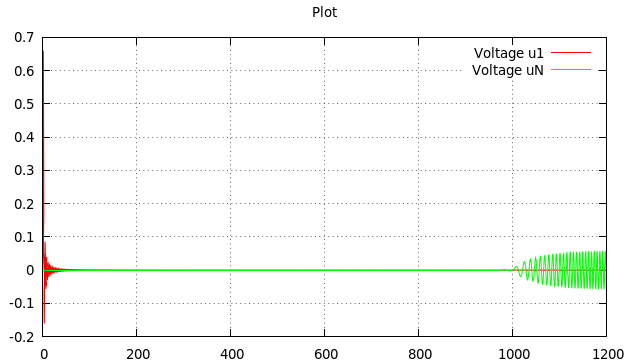
\includegraphics[width=\linewidth]{lcline-pd}
\end{minipage}\hfill
\begin{minipage}{0.5\textwidth}
\centering
 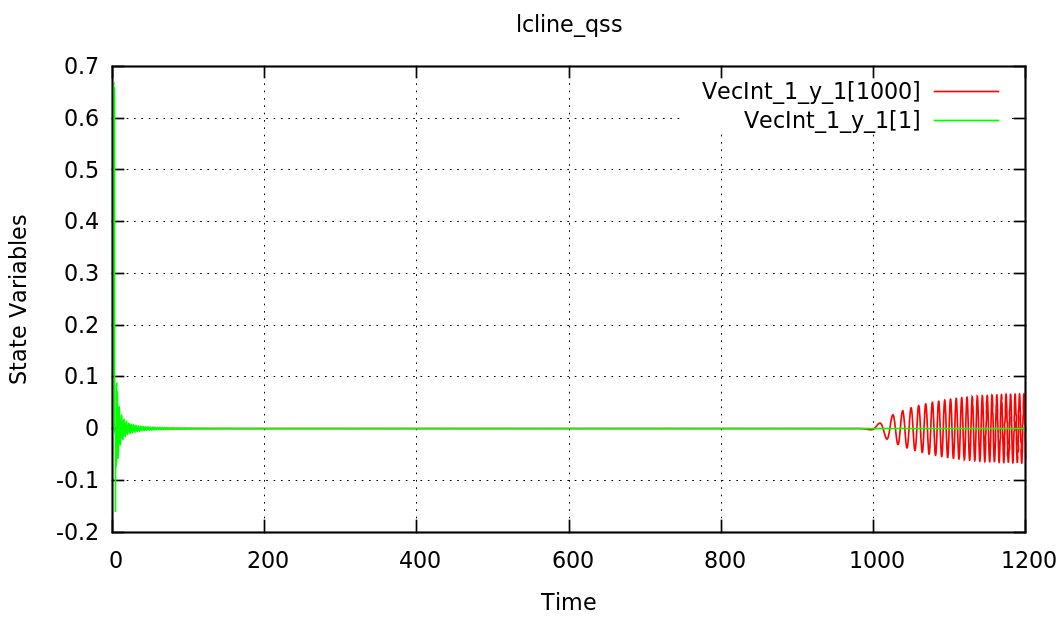
\includegraphics[width=\linewidth]{lcline-qss}
\end{minipage}
\end{figure}

\section{Inversores Lógicos}
	El siguiente modelo representa una cadena de $m$ inversores lógicos, 

\begin{align*}
\dot{\omega}_1 & = U_{op} - \omega_1(t) - \Upsilon g (u_{in}(t), \omega_{1} (t))    \\
\dot{\omega}_j & = U_{op} - \omega_j(t) - \Upsilon g (\omega_{j-1}(t), \omega_{j} (t)) \textrm{ donde $j = 2, 3, .., m$}
\end{align*}


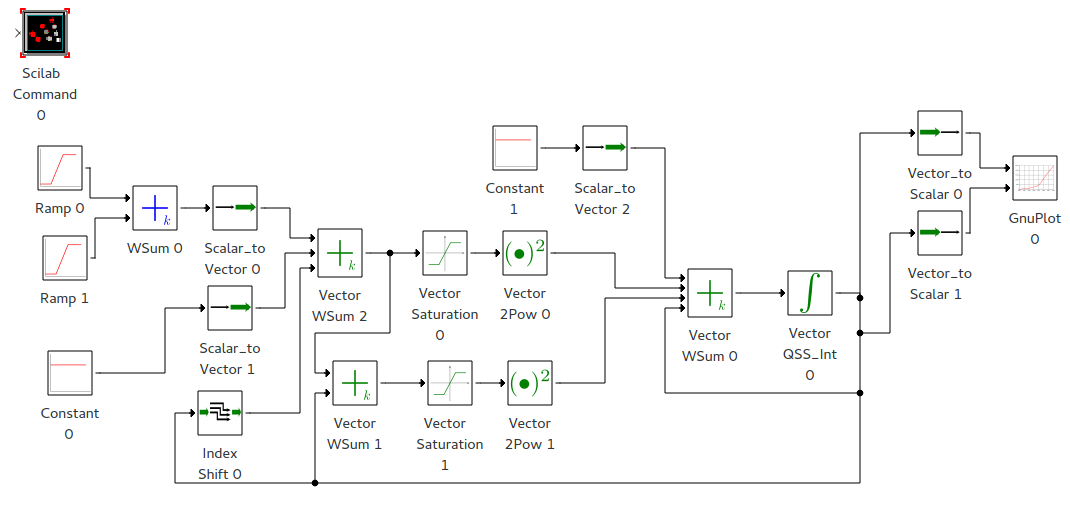
\includegraphics[width=0.75\linewidth]{inverters}

\begin{figure}[H]
\centering
\begin{minipage}{0.5\textwidth}
\centering
 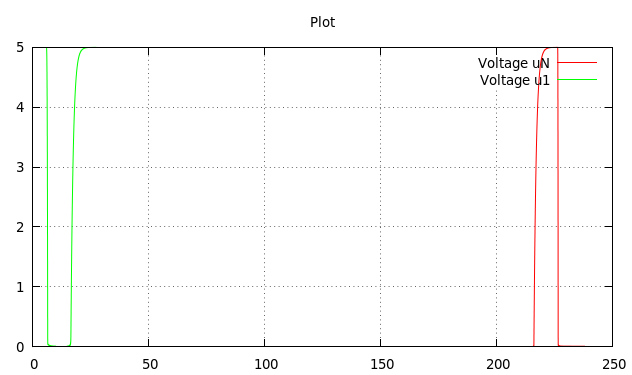
\includegraphics[width=\linewidth]{inversers-pd}
\end{minipage}\hfill
\begin{minipage}{0.5\textwidth}
\centering
 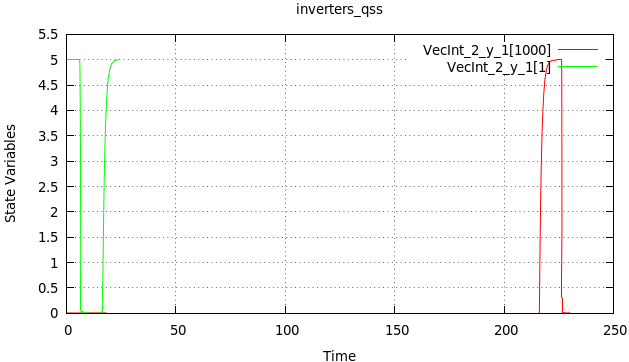
\includegraphics[width=\linewidth]{inversers-qss}
\end{minipage}
\end{figure}

\section{Advection-diffusion-reaction}
	El modelo de equaciones Advection-diffusion-reaction (ADR) provee las bases para describir fenomenos de tranferencias de calor y masa, donde la cantidad de interes $u(x,t)$ puede ser temeratura en la conducción de calor o concentración de una sustancia química.

La ecuación 
\begin{equation*}
\frac{du(x,t)}{dt} + a \frac{du(x,t)}{dx} = d\frac{d^2u(x,t}{d^2x} + r(u(x,t)^2 - u(x,t)^3)
\end{equation*}
corresponde al modelo ADR, donde $a$,$d$ y $r$ son parametros expresando coeficientes de advección, difusión y reactión

 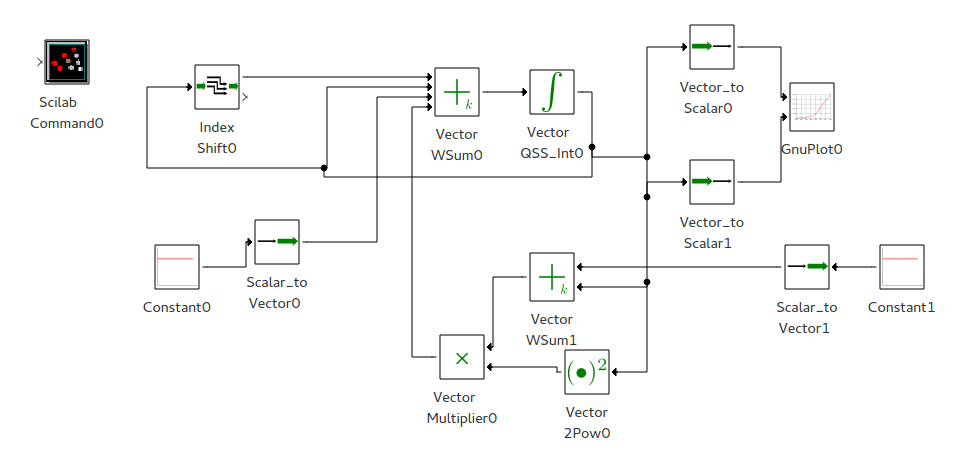
\includegraphics[width=0.75\linewidth]{adr-pwd}

\begin{figure}[H]
\centering
\begin{minipage}{0.5\textwidth}
\centering
 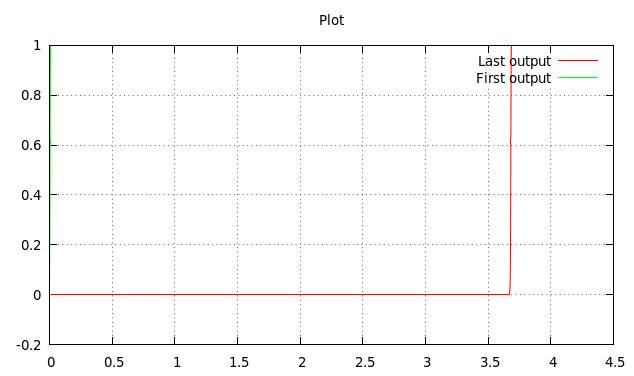
\includegraphics[width=\linewidth]{adr-pd}
\end{minipage}\hfill
\begin{minipage}{0.5\textwidth}
\centering
 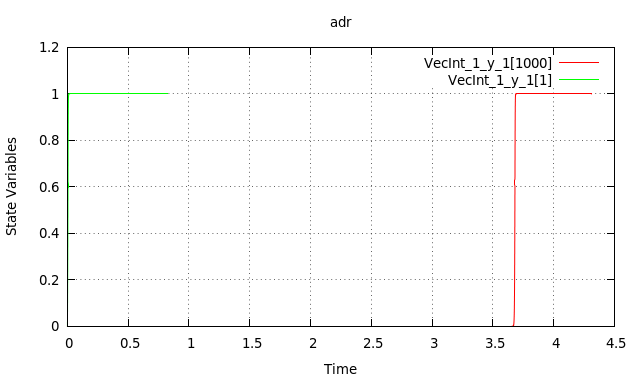
\includegraphics[width=\linewidth]{adr-qss}
\end{minipage}
\end{figure}

\section{Convertidor de Voltaje}
	El siguiente modelo es un tipo de convertidor DC - DC que obtiene a su  salida  un  voltaje  continuo  menor  que  a  su entrada, manteniendo una una  alta eficiencia (superior al 95\% con circuitos integrados) y autoregulación.

\begin{align*}
\frac{di_{L}}{dt} & = \frac{-u_{C} - R_D i_D }{L}\\
\frac{du_C}{dt} & =i_D \frac{i_D}{C} - \frac{u_C}{R_L C }
\end{align*}
donde
\begin{align*}
i_D & = \frac{R_s i_L - u_C - U }{R_D + R_s}
\end{align*}


\begin{figure}[H]
\centering
 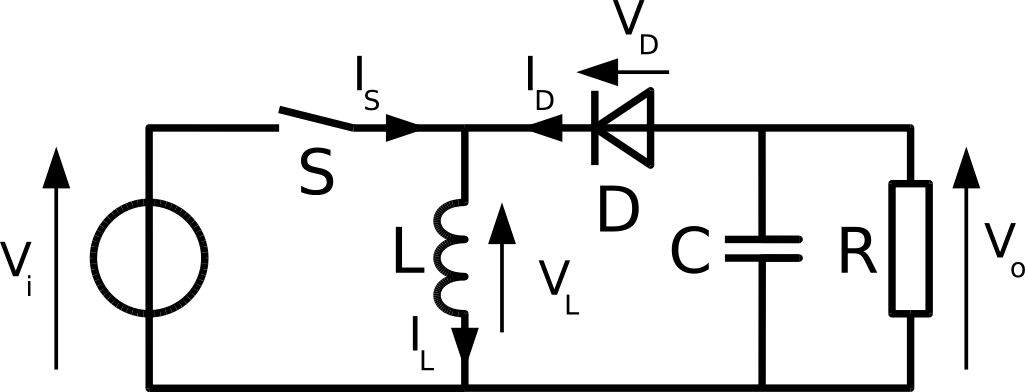
\includegraphics[width=.60\linewidth]{Buckboost_conventions}
 \caption{Esquema electrico de convertidor de voltaje}
\end{figure}

\begin{figure}[H]
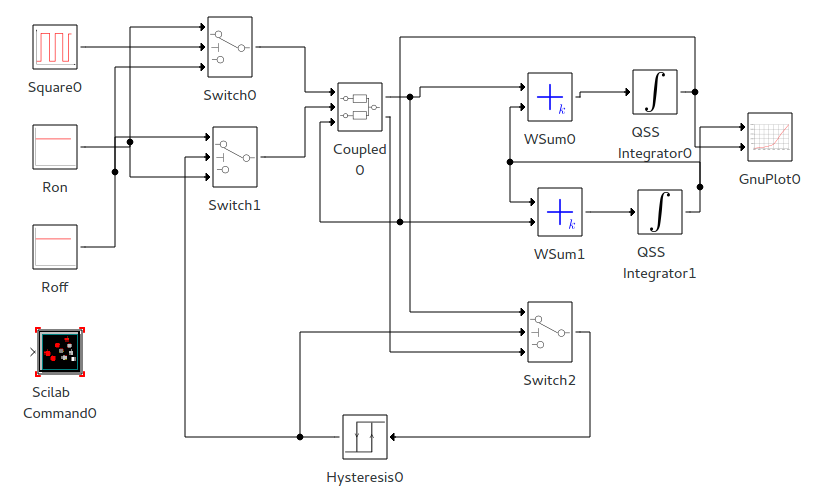
\includegraphics[width=0.75\linewidth]{buck_disk}
\caption{Modelo Convertidor de voltaje}
\end{figure}

\begin{figure}[H]
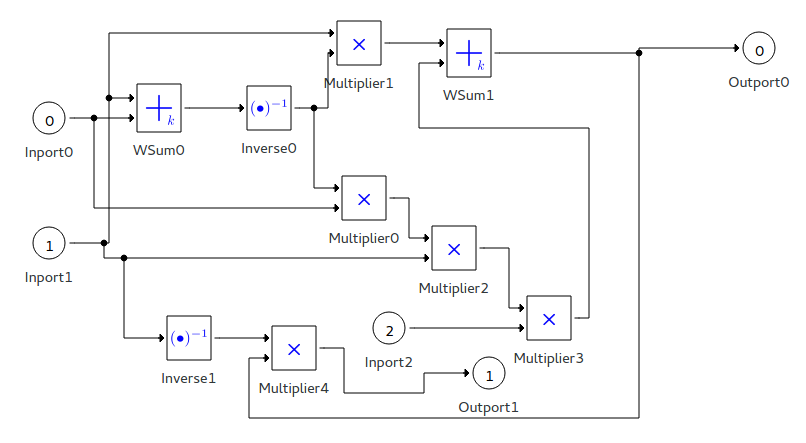
\includegraphics[width=0.75\linewidth]{buck_disk_coupled0}
\caption{Coupled0 (Incluido en Convertidor de voltaje)}
\end{figure}

\begin{figure}[H]
\centering
\begin{minipage}{0.5\textwidth}
\centering
 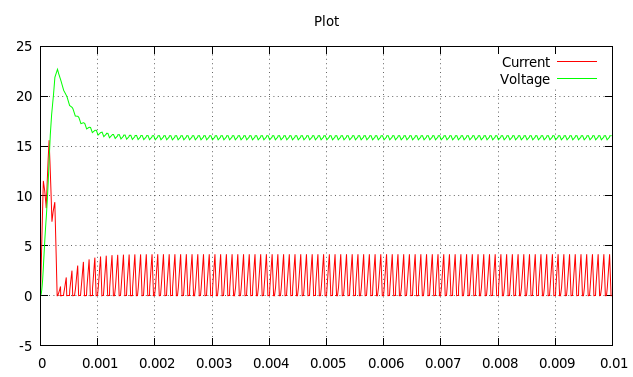
\includegraphics[width=\linewidth]{buck_disk-pd}
\end{minipage}\hfill
\begin{minipage}{0.5\textwidth}
\centering
 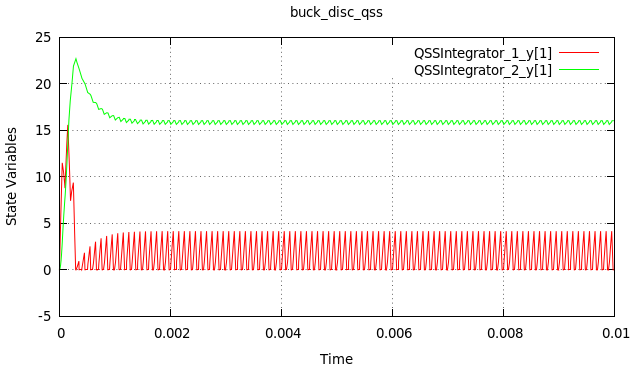
\includegraphics[width=\linewidth]{buck_disk-qss}
\end{minipage}
\end{figure}

\section{Ecuaciones Lotka-Volter}

	El sistema de ecuaciones Lotka-Volter, es un sistema de ecuaciones diferenciales de primer orden, no lineales, utilizadas para describir dinámicas de sistemas biológicos en el cual dos especies interactúan, una como presa y otra como depredador, se definen como:

\begin{align*}
\frac{dx}{dt} & = x(\alpha - \beta y)\\
\frac{dy}{dt} & =y(\gamma - \delta  x)
\end{align*}

donde:
\begin{itemize}
	\item y es el número de algún predador (por ejemplo, un lobo);
    \item x es el número de sus presas (por ejemplo, conejos);
    \item t representa el tiempo; y
    \item $\alpha$, $\beta$, $\gamma$, $\delta$ son parámetros que representan las interacciones de las dos especies.
\end{itemize}

	Este sistema es representado por el modelo siguiente:

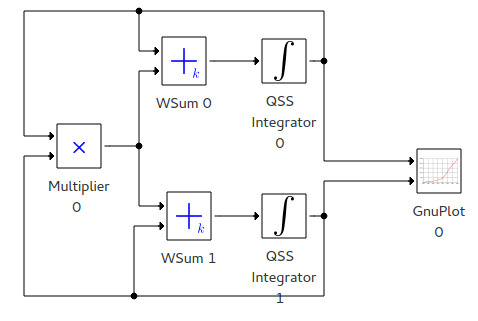
\includegraphics[width=0.75\linewidth]{lotka_voltera_pwd}

\begin{figure}[H]
\centering
\begin{minipage}{0.5\textwidth}
\centering
 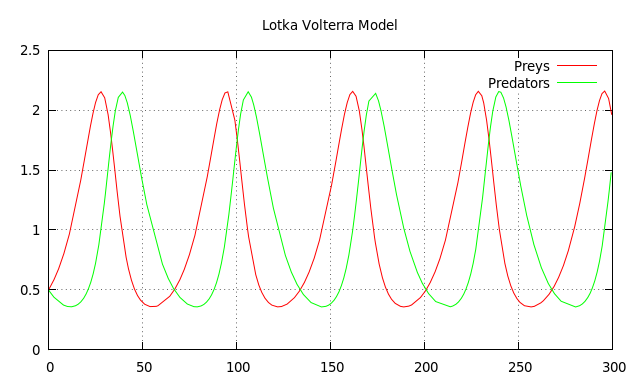
\includegraphics[width=\linewidth]{lotka_voltera-pd}
\end{minipage}\hfill
\begin{minipage}{0.5\textwidth}
\centering
 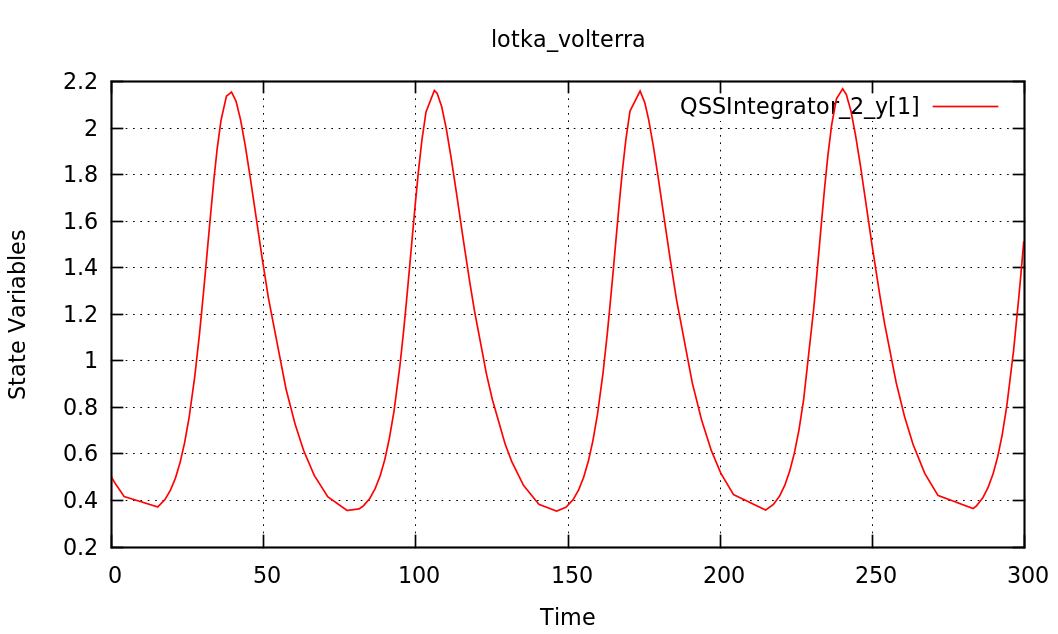
\includegraphics[width=\linewidth]{lotka_voltera-qss}
\end{minipage}
\end{figure}

\section{Resultados}

	Las pruebas fueron realizadas en una PC Intel\textsuperscript{\textregistered} Core\textsuperscript{TM} i7-3632QM CPU @ 2.20GHz con 16 GB de memoria RAM. Los tiempos observados no deben ser considerados 
	como absolutos ya que variaran de un sistema a otro, pero las mejoras relativas en los tiempos de ejecución deberían mantenerse.

	Los resultados obtenidos son los tiempos observados luego de ejecutar la simulación en PowerDEVS (P.DEVS) y QSS-Solver (QSS-S), ambas mediciones
	son reportadas por los motores de simulación, en milisegundos (ms), todas las simulaciones utilizan el método de integración QSS3 excepto los que 
	se especifica LIQSS2.

\begin{table}[H]
\centering	
\label{my-label}
\begin{tabular}{llllll}
\toprule
{\bf Modelos}            &  {\bf P.DEVS(ms)} & {\bf QSS-S. (ms)} & {\bf Mejora (\%)} \\
\toprule
Lineas de Transmisión 1200s, N=1000     & 76402         & 34982.5         & 54          \\
Inversores(LIQSS2) 250s, N=1000   	& 25046         & 7694.44         & 69        \\
ADR(LIQSS2) 10s, N=1000 		& 6089          & 568.772         & 90        \\
Convertidor de Voltaje 0.01s,        	& 268           & 10.3802         & 96         \\
Lotka  Voltera 300s      		& 11            & 2.75132         & 81

% Mejora esta calculada a partir de 1 - qsssolver / pwdevs
%excepto indicado, se utiliza QSS3
\end{tabular}
\end{table}

	En la tabla se puede ver una mejora entre 54 y 96\% entre todos los modelos, y entre 54 y 90\% para los modelos vectoriales que son nuestro principal objetivo,
	ya que son la forma más simple de realizar grandes modelos, que es lo que esperaba dado que al cambiar de formalismo se evita todo los mensajes entre modelos 
	caracteristico del formalismo DEVS, además de aprobechar la velocidad del QSS-Solver.


\chapter{Conclusiones y Trabajos futuros}

\section{Conclusiones}

	En el presente trabajo se mostró, en detalles, la implementación de una conversión de modelos de PowerDEVS en modelos $\mu$-Modelica que permite un ahorro 
	en el tiempo de simulación cercana al 90\% en modelos grandes, mostramos como se mantiene los valores de la simulación a través de comparar las gráficas de 
	los resultados obtenidos.

\section{Trabajos Futuros}
	Para poder convertir una mayor variedad de modelos, en PowerDEVS, es necesario escribir más modelos en modelica.
	Para convertir modelos de tiempo real sera necesario expandir expandir el QSS-Solver para soportarlo.
	Para facilitar la integración se planeo integrar el conversor de forma que pueda ser ejecutado desde la interfaz gráfica de PowerDEVS, posiblemente con la opción de ejecutarlo en el QSS SOlver.
	Durante el desarrollo de este trabajo, la libreria modelicacc (http://sourceforge.net/projects/modelicacc/?source=directory ) , ha sido actualizada con un nuevo parser, el cual deberá ser remplazado.
	La expansión de variables vectoriales, donde los valores provienen de expresiones del entorno scilab, es siempre tratado como un valor escalar, y no como uno vectorial, para determinar como se lo debería tratar es necesario realizar un analisis de los tipos de las variables expandidas. Lo cual podria mejorar los mensajes de error en el caso de que se conecten modulos vectoriales con modulos escalares.

\appendix
\chapter{Modelos Creados}
A continuación mostramos los modelos $\mu$Modelica equivalentes a los modelos PowerDEVS, utilizados para realizar la comparación de performance:

\begin{listing}[H]    
     \caption{data/sources/constant\_sci.mo}\label{list:constant_sci.mo}
     \inputminted{modelica}{../../data/sources/constant_sci.mo}
\end{listing} 

\begin{listing}[H]    
	\caption{data/sources/pulse\_sci.mo} \label{list:pulse_sci.mo}
	\inputminted{modelica}{../../data/sources/pulse_sci.mo}
\end{listing} 

\begin{listing}[H]    
	\caption{data/sources/ramp\_sci.mo} \label{list:ramp_sci.mo}
	\inputminted{modelica}{../../data/sources/ramp_sci.mo}
\end{listing} 

\begin{listing}[H]    
	\caption{data/sources/square\_sci.mo} \label{list:square_sci.mo}
	\inputminted{modelica}{../../data/sources/square_sci.mo}
\end{listing} 

\begin{listing}[H]    
	\caption{data/qss/hysteretic.mo} \label{list:hysteretic.mo}
	\inputminted{modelica}{../../data/qss/hysteretic.mo}
\end{listing} 

\begin{listing}[H]    
	\caption{data/qss/inverse\_function.mo} \label{list:inverse_function.mo}
	\inputminted{modelica}{../../data/qss/inverse_function.mo}
\end{listing} 

\begin{listing}[H]    
	\caption{data/qss/qss\_integrator.mo} \label{list:qss_integrator.mo}
	\inputminted{modelica}{../../data/qss/qss_integrator.mo}
\end{listing} 

\begin{listing}[H]    
	\caption{data/qss/qss\_multiplier.mo} \label{list:qss_multiplier.mo}
	\inputminted{modelica}{../../data/qss/qss_multiplier.mo}
\end{listing} 

\begin{listing}[H]    
	\caption{data/qss/qss\_quantizer.mo} \label{list:qss_quantizer.mo}
	\inputminted{modelica}{../../data/qss/qss_quantizer.mo}
\end{listing} 

\begin{listing}[H]    
	\caption{data/qss/qss\_switch.mo} \label{list:qss_switch.mo}
	\inputminted{modelica}{../../data/qss/qss_switch.mo}
\end{listing} 

\begin{listing}[H]    
	\caption{data/qss/qss\_wsum.mo} \label{list:qss_wsum.mo}
	\inputminted{modelica}{../../data/qss/qss_wsum.mo}
\end{listing} 

\begin{listing}[H]    
	\caption{data/vector/IndexSelector.mo} \label{list:ndexSelector.mo}
	\inputminted{modelica}{../../data/vector/IndexSelector.mo}
\end{listing} 

\begin{listing}[H]    
	\caption{data/vector/vec2scalar.mo} \label{list:ec2scalar.mo}
	\inputminted{modelica}{../../data/vector/vec2scalar.mo}
\end{listing} 

\begin{listing}[H]    
	\caption{data/vector/scalar2vec.mo} \label{list:calar2vec.mo}
	\inputminted{modelica}{../../data/vector/scalar2vec.mo}
\end{listing} 

\begin{listing}[H]    
	\caption{data/vector/vector\_sum.mo} \label{list:ector_sum.mo}
	\inputminted{modelica}{../../data/vector/vector_sum.mo}
\end{listing} 

\begin{listing}[H]    
	\caption{data/vector/qss\_integrator\_vec.mo} \label{list:ss_integrator_vec.mo}
	\inputminted{modelica}{../../data/vector/qss_integrator_vec.mo}
\end{listing} 

\begin{listing}[H]    
	\caption{data/vector/index\_shift.mo} \label{list:ndex_shift.mo}
	\inputminted{modelica}{../../data/vector/index_shift.mo}
\end{listing} 

\begin{listing}[H]    
	\caption{data/vector/qss\_sum\_vec.mo} \label{list:qss_sum_vec.mo}
	\inputminted{modelica}{../../data/vector/qss_sum_vec.mo}
\end{listing} 

\begin{listing}[H]    
	\caption{data/vector/qss\_multiplier\_vec.mo} \label{list:ss_multiplier_vec.mo}
	\inputminted{modelica}{../../data/vector/qss_multiplier_vec.mo}
\end{listing} 

\begin{listing}[H]    
	\caption{data/vector/vector\_pow2.mo} \label{list:ector_pow2.mo}
	\inputminted{modelica}{../../data/vector/vector_pow2.mo}
\end{listing} 

\begin{listing}[H]    
	\caption{data/vector/hyst\_vec.mo} \label{list:yst_vec.mo}
	\inputminted{modelica}{../../data/vector/hyst_vec.mo}
\end{listing} 

\begin{listing}[H]    
	\caption{data/vector/vector\_sat.mo} \label{list:ector_sat.mo}
	\inputminted{modelica}{../../data/vector/vector_sat.mo}
\end{listing} 

\newpage


\nocite{*}

\bibliographystyle{unsrt}
\cleardoublepage

\phantomsection

\addcontentsline{toc}{chapter}{Bibliografía}
\bibliography{tesina_luciano}


\end{document}
